\documentclass[10pt,journal,compsoc]{IEEEtran}

\usepackage[T1]{fontenc}
\usepackage[utf8]{inputenc}

\usepackage{graphicx}
\usepackage[export]{adjustbox}

\usepackage{cite}

\graphicspath{{./figures/}}
\usepackage{subcaption}

\usepackage{amsthm, amsmath, amsfonts}
\interdisplaylinepenalty=2500

\usepackage{algorithmic}
\usepackage{array}
\usepackage{url}

\hyphenation{}

\newcommand{\ts}{\textsuperscript}

\begin{document}
\title{Dyr, a Program for Bayesian Inference of Language Phylogenies}

\author{Student Name: J.G. Byrne\\Supervisor Name: Professsor M.J.R. Bordewich\\
Submitted as part of the degree of MEng Computer Science to the\\
Board of Examiners in the Department of Computer Sciences, Durham University
}


\markboth{DURHAM UNIVERSITY, DEPARTMENT OF COMPUTER SCIENCE}%
{Shell \MakeLowercase{\textit{et al.}}}

\IEEEtitleabstractindextext{%
\begin{abstract}
Bayesian statistics provide a powerful framework for inferring the evolutionary history of language families from lexical data, a problem which is made computationally tractable by Markov Chain Monte Carlo (MCMC) algorithms. We present Dyr, a simple yet capable new system for Bayesian inference, and use it to perform novel state-of-the-art analyses of the Indo-European language family. 
\end{abstract}

\begin{IEEEkeywords}
Bayesian Inference, Markov Processes, Linguistics, Indo-European
\end{IEEEkeywords}}

\maketitle
\IEEEdisplaynontitleabstractindextext
\IEEEpeerreviewmaketitle

\IEEEraisesectionheading{\section{Introduction}\label{sec:introduction}}

\IEEEPARstart{L}{anguages} evolve over time. Some of these changes are phonetic or grammatical, but many are lexical (changes in the vocabulary). Words are forgotten and replaced, sometimes by other words that have changed meaning, and sometimes by borrowings from other languages.\footnote{For example, the Old English word \textit{dēor} was displaced by the French 'animal', and survives only in the narrower sense 'deer'. However, the equivalent word in Danish, \textit{dyr}, whence this project name, retains the older meaning. Both words derive from Proto-Germanic \textit{*deuzą}, ultimately from Proto-Indo-European \textit{*d\ts{h}wes}, meaning 'breath'.} Occasionally, some speakers of a language will come to speak so differently to the others that the groups can no longer understand each other, and the language splits in two.

Scholars have noticed similarities between languages for millenia. In the 18\ts{th} century, the field of comparative linguistics was born, which seeks to systematically reconstruct the historical relationships between languages. The early comparative linguists observed that while languages can evolve, sunder, and go extinct, they rarely merge, and are never created anew. Therefore, from the 19\ts{th} century onwards it became \textit{de rigeur} to describe language descent with evolutionary trees, or `phylogenies', and though not without criticism, this model remains predominant in linguistics to this day.

Historically, constructing phylogenies has been a job for humans, being based on the judgement of expert scholars with deep knowledge of languages ancient and modern. Although fruitful, this approach is naturally susceptible to human biases and oversights. It also provides no way to determine the age of unattested ancestor languages other than the (admittedly finely-honed) intuition of learned intellectuals.

The problem of ancestral dating is of particular relevance to Indo-European, the largest and most studied language family in the world. Encompassing nearly all of the languages of Europe and a great many in Western Asia and India, the challenge of reconstructing the history of this vast grouping has captivated comparative linguists since the advent of the discipline. And yet, one central question is still to be conclusively answered: where and when was Proto-Indo-European (PIE; the ancestor of all Indo-European languages) originally spoken? Two main theories abound. The first, known as the `Kurgan' hypothesis, postulates an \textit{Urheimat} (original homeland) in the Pontic-Caspian steppe north of the Black Sea\cite{gimbutas1974gods}.\footnote{A \textit{kurgan} is a tumulus or burial mound. This theory is associates the spread of Indo-European with warlike tumulus-building charioteers.} Conversely, the second proposes an origin in Anatolia\cite{renfrew2001anatolian}.\footnote{This rather more sedate theory suggests a gradual proliferation of Indo-European in tandem with the spread of agriculture} The crucial difference between the two theories is that while the former ascribes a time depth of 6000 years to PIE, the latter hinges on it being considerably more ancient, at approximately 8500 years old. A reliable estimate for the age of PIE - that is, the root age of the Indo-European language tree - could therefore be potent evidence for one theory over the other.

Since the millenium, researchers have adopted a new method to analyse language families in general and Indo-European in particular -- Bayesian inference. By re-appropriating software designed to analyse genetic data and construct biological evolutionary trees, they have successfully inferred plausible dated phylogenies from large vocabulary databases. Such research feels tantalisingly close to an objective solution to linguistic enigmas such as that of Indo-European provenance.

However, in reality, the human factor still plays a role. Bayesian methods require the specification of prior distributions, the choice of which can radically affect the results of the inference. For research to be rigorous and reliable, priors should be chosen carefully and properly justified.

Yet much study in the relatively small field of `Bayesian Phylolinguistics' falls short of this mark. Priors are often chosen seemingly out of habit or convention. Such laxness poses particular dangers when these conventions have their origins in bioinformatics; a model which is sensible in the context of biological evolution may not be so logical when applied to languages.

We suggest that one reason for this tendency is the continued reliance on large, featureful bioinformatics software packages like BEAST2 and MrBayes. Any dedicated support for linguistics in these programs tends to be something of an afterthought, and their intimidating size makes them hard to understand in their totality. Therefore, we submit that to step out of the shadow of the older, larger discipline, it is desirable for Bayesian phylolinguistics to have its own dedicated software package.

The objective of our research was to build such a software package. Our key aims were for it to be high-performance and efficient (that is, to minimise repeated computation), to be modern and extensible, and to support practical features that are necessary for contemporary Bayesian phylolinguistics. Such features include prior likelihood models based on Coalescent Theory, topology constraints on both clade inclusion and clade ancestry, and support for data interchange standards such as NEXUS and Newick.

We thus present \textit{Dyr}, a new program for Bayesian inference of language phylogenies. \textit{Dyr} is written in the modern systems language Rust, is small enough that its source code may be read and understood in a day, and offers only the features required for linguistic applications. Nonetheless, it is designed to be efficient and easily extensible. 

In section \ref{sec:related} of this paper we will describe the research that has led up to the contemporary understanding and usage of Bayesian phylogenetic inference, and in particular its application to Indo-European. We will also discuss existing inference software. In section \ref{sec:methods} we will describe the theoretical principles underpinning Bayesian inference in general and \textit{Dyr} in particular. We will also discuss the suitability of particular prior models to phylolinguistic research, and justify our own choice of model. 

This theoretical grounding will then be built upon in section \ref{sec:implementation}, where we discuss the structure of the \textit{Dyr} system. We describe the techniques we used to faithfully implement our theoretical models, while at the same time achieving our technical goals of simplicity, efficiency, and extensibility.

In section \ref{sec:results}, we present the results of our application of \textit{Dyr} to the benchmark Indo-European problem domain. We demonstrate the reliability of our software by showing that it produces similar results to Chang et. al when performing similar analyses. We also perform our own novel analyses, using our favoured prior model from \ref{sec:methods}. Based on the results of these analyses, we conclude that the Steppe hypothesis for the Indo-European \textit{Urheimat} is the most plausible, re-affirming the results of Chang et. al.   

Finally, in section \ref{sec:conclusion}, we summarise and reflect upon the outcomes of our work and re-iterate our hope that going forward, \textit{Dyr} can serve as a worthy platform for trialling novel phylogenetic methods with direct linguistic justification and application.

\section{Related Work}\label{sec:related}

The most general description of the problem that our work seeks to solve, and indeed that the entire field of Computational Phylogenetics is broadly centered around, is that it is the task of finding the tree or distribution of trees that best fits a given dataset, for some definition of `best fit'.

However, for as long as researchers have tried to tackle this problem with computational methods, they have quickly run up against firm combinatorical realities. The number of possible topologies - not even considering branch lengths - for a rooted binary tree with 52 leaves, the smallest size of tree we consider in our analyses, is on the order of $10^{80}$.\cite{felsenstein2004inferring}

One widely-used approach for optimising phylogenetic trees from genetic data has historically been the criterion of maximum parsimony; searching for the tree that minimises the number of mutations for a set of data. However, besides being an extremely hard search problem, this approach was criticised for ineffectively modelling evolutionary realities.

An alternative method is to use a likelihood model that describes a probability distribution over the space of possible trees. This approach has some noted advantages, not least that it allows the application of techniques such as the `relaxed clock', which allows evolutionary rates to vary.

A likelihood model is of little use without some way of sampling the probability distribution it implies; it is for this purpose that the family of algorithms known as Monte Carlo Markov Chain, or MCMC, was devised. The foundational work in this field was the creation of the Metropolis algorithm in the 1950s, which was later generalised by Hastings in 1970. However, the first application of MCMC to phylogenetics came later, in the 1990s, when hardware advances made the technique feasible for larger parameter spaces.

The elegant property that makes MCMC processes so attractive is their asymptoptic convergence on a defined stationary distribution over a parameter space. However, this convergence can be extremely slow if the proposal distribution is misconfigured; a tendency to take both steps that are too small and too large can bring convergence grinding to a halt. Tuning the proposal distribution to achieve consistent and rapid convergence can in practice be more of an art than a science.

Nonetheless, the fact that MCMC approximates a probability distribution and doesn't simply find a maxmima is a key advantage over traditional heuristic search. One can take `snapshots' from a chain during its execution and use them afterwards to create `summary' phylogenies, which combine the median values of various parameters to yield a candidate phylogeny that better represents the overall distribution than a simple maxima.

For example, the Maximum Clade Credibility (MCC) technique, which we use to summarise our analyses, is attractive since it yields a tree whose topology is strongly supported by a relatively large volume of probability density.

\subsection{Inferring Linguistic Phylogenies}

The first serious attempt to use statistical methods to investigate language phylogenies was made by Morris Swadesh in the 1950s. His `glottochronology' model -- which assumed a constant global rate of change -- had limited practical utility, but his ideas were foundational to more sophisticated subsequent attempts\cite{swadesh1955towards}. In particular, the concept of the Swadesh list, a collation of basic and universal word-semantics, underlies the lexical trait analysis used in quantitative historical linguistics today -- including in this report.

The first notable paper to use the MCMC technique to infer the posterior distribution of a linguistic phylogeny was Gray and Atkinson's groundbreaking 2003 study. Their analysis of the Indo-European family, which employed the forerunner of the modern IELEX dataset, lent robust support to the Anatolian hypothesis.\cite{gray2003language} This research was reinforced by the later results of Bouckaert et al.\cite{bouckaert2012mapping}\cite{bouckaert2013correction}, who used an updated dataset, and tested an alternative trait model devised by Nicholls and Gray\cite{nicholls2008dated} requiring that cognate traits arise just once in a phylogeny, again finding strongest support for an Anatolian origin.

This trend was bucked by Chang et al., who built upon the work of Bouckaert et al. with the key addition of novel prior constraints on tree topology.\cite{chang2015ancestry} In particular, they mandated that certain languages be effectively ancestral to others in the tree; for example, Old English is necessarily positioned as a direct ancestor to English. Their intention was to correct for a phenomenon that they dubbed `jogging'. Without ancestry constraints, an ancestral interior node will be postulated that is older than both a modern language and its more ancient ancestor.

This is undesirable for two reasons. Firstly, the tree distance between the two languages will be substantially longer than should actually be the case. This causes the Bayesian process to infer lower average evolutionary rates and thus an older root age for the tree. Secondly, it results in phylogenies which are simply not reconcilable with linguistic realities. If it is a known fact that there is a direct line of descent between a pair of languages then one cannot consider any conclusions drawn from a model that does not reflect this fact to be reliable! With these constraints imposed, and with some corrections applied to the Bouckaert et al. dataset, Chang et al. found the strongest support for the Steppe hypothesis.

Since the publication of the Chang et al. study, futher research has questioned the necessity of such constraints. Rama suggested that similar results to those obtained by Chang et al. could be obtained without ancestry constraints by usage of a Uniform tree prior.\cite{rama2018three} Rama astutely observed that the population size parameter of the Coalescent prior does not have an obvious interpretation in the context of language evolution, but neglected to apply the same standard of justifiability to the Uniform prior. This is in spite of the clear pitfalls of the Uniform prior; namely, that it implies a language family evolves as a collective whole, rather than evolution being a process happening largely independantly in each individual language.

However, his work does serve to highlight the potential for further investigation into the bread-and-butter of phylogenetic inference; prior distributions and substitution models. In particular we believe Rama's work demonstrates a neccessity for research into tree prior models that are empirically successful at replicating known results and also have sound linguistic justification. 

\subsection{Extant Software}

Bayesian phylogenetic inference is dominated by two large software packages, MrBayes\cite{ronquist2012mrbayes} and BEAST 2\cite{bouckaert2014beast}. The former is written in C while the latter uses Java -- languages which lack features that many modern programmers value. Both packages are extremely featureful, but many of these features are inappropriate in a linguistics context or are simply inapplicable. The size of these software packages makes them hard to study and modify; for example, MrBayes has nearly 100,000 lines of C code, of which 20,000 are the MCMC implementation alone.

Both BEAST 2 and MrBayes were originally written with Bioinformaticians as the target users; to my knowledge \textit{Dyr} is the first Bayesian inference package designed from the ground-up with phylolinguistics as the primary use-case. \textit{Dyr} follows the lead of both these software packages by using the BEAGLE3 library for hardware-accelerated computation of likelihoods.\cite{ayres2019beagle}

We have stated that \textit{Dyr} is written in the systems language Rust. Although growing rapidly in popularity, Rust is a young language, and remains a small player compared to such titans as C++ and Java. We will therefore briefly outline the attractive features of Rust that led us to choose it for our project.

One of our technical objectives was for \textit{Dyr} to be efficient, and on this point Rust made a good fit, since it is a compiled language with near-zero runtime overhead and no garbage collection. Another objective was pain-free extensibility, which we achieved through usage of Rust's modern and ergonomic features such as Algebraic Data Types and Closures. These features allowed us to design elegant and intuitive abstractions, which can be simply and cleanly built upon to add new functionality, as we shall demonstrate in sections \ref{sec:implementation} and \ref{sec:results}. Finally, Rust provides superb C interoperability, via native support for C FFI and automatic binding generation with \texttt{bindgen}. This was extremely helpful in allowing us to make use of the high-performance BEAGLE 3 library in \textit{Dyr}.

\section{Methods}\label{sec:methods}

The aim of phylogenetic inference is to determine which phylogenies are most likely given a particular evolutionary model and a set of known data. This is known as assessing the `posterior likelihood'. In a linguistics context, the known data is typically `lexical trait data' -- that is, information about the vocabulary of the languages in question. The evolutionary model, which in Bayesian terms provides our `prior likelihood', encapsulates our beliefs about how likely languages are to diverge and how rapidly their vocabulary changes. To allow our inferred phylogeny to best fit the signal present in the data, we also infer some parameters of our evolutionary model, though these too are subject to their own prior likelihood distributions.

The space of possible parameterisations is very large and it is not typically possible to analytically determine the maxima of the posterior likelihood distribution. Therefore, it is hard to gain an understanding of the shape of the posterior; to discern the regions in paramater space with the highest likelihood density. However, Bayes' theorem allows us to assess the posterior likelihood of any specific choice of parameterisation given the data. We therefore use MCMC to iteratively step through the space of possible parameterisations, with a preference for augmentations to the parameterisation that improve the posterior likelihood. It is provable that the long-run outcome of this process will be to simulate the desired posterior distribution.

In this section, we will first explain how lexical trait databases are compiled. We will then discuss how the posterior likelihood is defined in terms of the marginal and prior likelihood distributions, and how these distributions are themselves computed. Finally, we will outline the Metropolis-Hastings algorithm; the means by which the MCMC process itself is implemented.

\subsection{Lexical Trait Data}

The primary evidence used to infer linguistic phylogenies is lexical trait data. In principle, many different linguistic features could be appropriated to inform Bayesian inference, but for both principled and pragmatic reasons the vast majority of analyses use lexical data. In particular, the class of traits used in our datasets is what Chang et al. termed \textsc{Root Meaning} traits. These traits can be described as tuples in the form (\textit{ root },\;\texttt{semantic}\;). A \textsc{Root Meaning} trait is binary; either present or absent for a given language. A given trait is present in a language if that language has a common word for the \texttt{semantic} that derives from the \textit{root}. For example, the Irish word for a \texttt{fish} is `iasc', which like the English `fish', comes from the Indo-European root \textit{*peysk-}. So the trait (\textit{ *peysk- },\;\texttt{fish}\;) is present in both Irish and English. However the Greek word for \texttt{fish} is `ikhthus', which is believed to derive from the root \textit{*d\ts{h}g\ts{h}u-}. Therefore the trait is absent in Greek.

The IELEX database, upon which we shall base our analyses, includes hundreds of these traits, and is the gold-standard source of lexical data for Indo-European. In particular, we use the subsets of IELEX constructed by Chang et al., termed \textsc{Narrow}, \textsc{Medium}, and \textsc{Broad}, containing 52, 82, and 94 languages respectively. In our Bayesian inferences, as is typical, languages will correspond to the leaves -- also known as tips -- of our phylogenies.

\subsection{Defining the Posterior Distribution}

Bayes' theorem is stated as follows:
\begin{equation}
    Pr(A\;|\;B) = \frac{Pr(B\;|\;A) \cdot Pr(A)}{Pr(B)}
\end{equation}

In the context of phylogenetic inference, we seek to infer the probability distribution of possible parameterisations given the observed data. Therefore $Pr(B)$ corresponds to $Pr(x)$, the probability of the observed trait data $x$. We need not know what it is equal to since it is constant and the MCMC algorithm only deals with ratios of likelihoods. Meanwhile, $Pr(A)$ corresponds to $Pr(\Gamma)$, the prior likelihood of a given parameterisation $\Gamma$, which is defined more thoroughly as follows:
\begin{align*}
    \Gamma &= (\psi, \omega, \lambda)\\
    \psi   &= \text{parameters describing a dated tree}\\
    \omega &= \text{parameters of the prior model for dated trees}\\
    \lambda&= \text{parameters of the prior model for trait evolution}
\end{align*}
We thus derive equation \eqref{eqn:posterior}. The posterior likelihood is proportional to the likelihood of the data given the parameterisation -- known as the marginal likelihood -- multiplied by the prior likelihood of the parameterisation. This is a proportionality because we do not know the value of $Pr(x)$, and also because we do not require that our prior distributions sum to 1 (for this reason we notate them with $f$ instead of $Pr$).
\begin{equation}\label{eqn:posterior}
    Pr(\Gamma\;|\; x) \propto Pr(x\;|\;\psi, \omega, \lambda) \cdot f(\psi\;|\;\omega) \cdot f(\omega) \cdot f(\lambda)
\end{equation}

We define $\psi = (\tau, \delta)$, where $\tau$ is the topology of the tree and $\delta$ is the branch lengths. We consider the node or nodes with the longest path from the root to be at $t = 0$ and therefore in the present day, while all other nodes are understood to be at some $t > 0$, corresponding to their distance from the present in years. Naturally, any interior node is required to be older than both its children.

\subsection{Marginal Likelihood}

Although Bayes' theorem absolves us of the need to directly calculate the posterior, we must still calculate the marginal likelihood. Conceptually speaking, this is the sum likelihood of the data $x$ being observed at the tips, across all possible trait assignments, as adjudged under a specified process of trait evolution we call the substitution model. A trait assignment, to be clear, can be understood as an assignment of an array to every node in the tree, wherein each array contains a bit of binary data for every trait, symbolising the presences or absence of that trait. Therefore, the sum across all trait assignments is the sum across every possible combination of trait presence-and-absence across every node of the tree (excepting the observed trait data at the tips). It is not hard to see that the number of permutations that need to be considered is enormous.

\subsubsection{Felsenstein's Algorithm}

At first glance, then, this calculation sounds intractable. However it can in fact be computed with a divide-and-conquer method called Felsenstein's algorithm. We will first give a high-level overview of this algorithm and then go on to describe it in more detail.

For each trait, we first define the trait's likelihood at the tips, based on the observed data. Then we work our way up the tree, at each interior node deriving the `partial' likelihoods of each possible state for that trait, using the partial likelihoods of the node's two children. When we reach the root, the likelihood is no longer partial, and we can therefore calculate an overall likelihood for the trait, which is equal to the sum across all assignments. The marginal likelihood of the tree is then simply the product of all the individual trait likelihoods.\cite{felsenstein2004inferring}

Equation \eqref{eqn:felsenstein} below gives a formal definition of Felsenstein's algorithm. We denote the likelihood of a node $x$ having state $t$ for the trait $i$ as $L_x^{i}(t)$, and it is defined separately for leaf nodes $\ell$ and for interior nodes $a$. It's worth remembering that for our purposes the set of states is simply $t \in \{0, 1\}$, but the algorithm is best understood in its full generality. When a leaf node $\ell$ has recorded data for trait $i$, the value $x_\ell^{i}\left[\;t\;\right]$ is $1.0$ for the observed state $t$ and $0.0$ otherwise. When instead, the data is missing, the likelihood is split evenly between all values of $t$. For an interior node $a$, the likelihood of having state $t$ for the trait $i$ is calculated based on the product of the sum likelihood across all possible ways $t$ can evolve along the branch to the left child $b$ and the equivalent calculation along the branch to the right child $c$. The evolution probability, denoted $Pr^i_{a,b}\left(u\,\vert\,t\right)$ for the left branch and $Pr^i_{a,c}\left(v\,\vert\,t\right)$ for the right, is the core calculation performed by the substitution model and is predicated on the parameters $\lambda$. Note how the likelihood is thus recursively `rolled-up' towards $r$, the root node of the tree.

\begin{equation}\label{eqn:felsenstein}
    \setlength{\jot}{12px}
    \begin{split}
        L_\ell^{i}(t) &= x_\ell^{i}\left[\;t\;\right] \\
        L_a^{i}(t) &= \left(\sum_uPr^i_{a,b}\left(u\,\vert\,t\right)L_b^{i}\left(u\right)\right)\left(\sum_vPr^i_{a,c}\left(v\,\vert\,t\right)L_c^{i}\left(v\right)\right) \\
        \mathcal{L}^{i} &= \sum_u \;\pi_u \cdot L_r^{i}\left(u\right) \\
        \mathcal{L} &= \prod_i \;\mathcal{L}^i
    \end{split}
\end{equation}

We denote the root likelihood across all states of trait $i$ as $\mathcal{L}^{i}$. The calculation required is a weighted average, with the weights being the stationary frequencies $\pi_u$, which will be discussed shortly along with the other parameters in $\lambda$.

Calculating the final likelihood is then a simple matter of taking the product of all of the per-trait root likelihoods. This value, $\mathcal{L}$, is the marginal likelihood -- equivalent to the term $Pr(x\;|\;\psi, \omega, \lambda)$ in equation \eqref{eqn:posterior}.

\subsubsection{Substitution Model and Trait Evolution}

We will now explain how the substitution model is used to calculate the probability of a state $t$ evolving to a state $u$ along a given edge of a tree. Let us state upfront the parameters of the model:

\begin{align*}
    \lambda &= (\mu,\;\pi,\;\alpha,\;\beta,\;\phi)\\
    \mu &= \text{Substitution base rate}\\
    \pi &= \text{Stationary frequencies: } \pi_0, \pi_1 \in \left(0, 1\right) : \pi_0 + \pi_1 = 1.0\\
    \alpha &= \text{Shape for Among Site Rate Variation (ASRV)}\\
    \beta &= \text{Shape for Among Branch Rate Variation (ABRV)}\\
    \phi &= \text{ABRV Rate Assignments}
\end{align*}

The core of the substitution model is the rate matrix, which describes the rates at which states mutate into each other. These matrices can be quite complex, but we opt for the simplest choice, the Generalised Time Reversible (GTR) model.\footnote{Chang et al. calls this the Restriction Site Character (RSC) model; the two are equivalent in the case of binary traits.} We have already seen how the stationary frequencies $\pi_0$ and $\pi_1$ influence the likelihood calculation, but they are also at the heart of the binary GTR rate matrix. 
\begin{equation}\label{eqn:ratematrix}
\textbf{Q} = \frac{1}{2\pi_0\pi_1} \begin{bmatrix}
-\pi_1 & \pi_1\\
\pi_0 & -\pi_0
\end{bmatrix} \text{ \ given that \ } \pi_0 + \pi_1 = 1.0
\end{equation}

As the length of time over which a trait evolves increases, the probability of it being in a state $u$ asymptopically approaches $\pi_u$, and the state it was initially in becomes irrelevant. To be more precise, for every branch $(a, b)$ in the tree $\psi$, for every trait $i$, the transition probabilities $Pr^i_{a,b}\left(u\,\vert\,t\right)$ are defined by the transition matrix $\textbf{P}^i_{a,b}$, where:

\begin{equation}\label{eqn:rate}
\textbf{P}^i_{a,b} = \exp\left(\textbf{Q} \cdot \delta_{a,b} \cdot \eta^i_{a,b}\right) \text{  \ where  \  } \eta^i_{a,b} = \mu \cdot \gamma_i \cdot \rho_{a,b}
\end{equation}

As previously stated, the value $\delta_{a,b}$ is the length (in years) of the branch $(a, b)$. The value $\eta^i_{a,b}$ is the rate for the trait $i$ on the branch $(a, b)$, calculated as the product of three rate parameters. The first rate,  $\mu$, is the base rate -- a global parameter that cancels out the units of the branch lengths and controls the overall rate of evolution. The second, $\gamma_i$, is the site rate,\footnote{The term `site' is a relic from bioinformatics, where traits typically correspond to specific sites on the genome} which is specific to this trait $i$. It is drawn from a Gamma distribution $\Gamma(\alpha, \frac{1}{\alpha})$. The third rate, $\rho_{a,b}$, is the branch rate, which is specific to this branch. It is drawn from a Log-Normal distribution $\log \mathcal{N}(-\frac{\beta^2}{2}, \beta^2)$. Both of these distributions have a mean of $1$, so regardless of their shapes the global average rate is equal to $\mu$. The choices of distributions are partly informed by implementation pragamatics and partly by the flexibility in shape that can be attained by modfications to $\alpha$ and $\beta$. \footnote{This paragraph abstracts quite significantly over the specifics of how these rates are actually chosen, which shall be discussed later.}

At this point the reader may be questioning the necessity of allowing rates to vary both across sites and and across branches. However there is a strong justification for both laxities. Variation in site rate is necessary because words vary greatly in their volatility. Certain common words, in particular numerals, change incredibly rarely. Others are considerably more susceptible to replacement. Equally, branch rates must be variable because languages evolve at dramatically different rates. A failure to account for this fact was the downfall of much early research into quantitiative historical linguistics. The classic (though by no means sole) example is the case of the Nordic languages; while Norwegians find Old Norse virtually incomprehensible, Icelanders can read it as easily as an Englishman can read Jane Austen. The reason for this is simply that the rate of change of Icelandic has been remarkably slow, while that of Norwegian has been reasonably fast.

\subsection{Prior Distributions}

The second part of equation \eqref{eqn:posterior} is the prior likelihood of the parameterisation. These terms express our baseline evolutionary model for phylogenies in general and language in particular.

The first prior term in \eqref{eqn:posterior} is $f(\psi\;|\;\omega)$, which expresses the prior likelihood of the tree $\psi$ conditioned on the set of parameters $\omega$. In turn, the parameters $\omega$ have their own prior distribution $f(\omega)$. Together, these terms fully implement the prior likelihood model for dated trees, informally known as the `tree prior'. The choice of tree prior is among the most impactful and contentious choices that a researcher needs to make when performing phylogenetic inference.

\subsubsection{Tree Constraints}

To be precise, the prior distribution over $\psi$ is actually composed of a general-purpose phylogenetic model and a set of dataset-specific constraints. We implement three such classes of constraints: tip calibrations, clade constraints, and ancestry constraints.

Tip calibrations constrain the ages of tips that are positioned at some depth in the past. They are implemented as windows of uniform prior density, with all times outside the window having zero prior likelihood. These calibrations are used to encode our convictions about the time periods in which ancient languages were used into the prior model, while giving the inference process freedom to infer the time-depth of these nodes if such a signal exists. As an example, in our Indo-European inferences, the well understood language of Old English has a relatively tight calibration window of (950, 1050) years before the present, while Tocharian B -- about which we know comparatively little -- has a wider window of (1200, 1500) years.

The second constraint class is clade constraints, which are improper priors that simply impose a very large likelihood penalty on topologies that do not contain a given clade. A clade, also known as a monophylectic group, is a set of taxa (i.e. languages) that are all more closely related to each other than they are to any other taxon. Intuitively, a clade is a group that can be pruned from the tree by snipping in exactly one place. Implementing such a constraint into a prior model is sensible when a clade has been established by scholars beyond any doubt.

The third constraint class is ancestory constraints, which are an extension of clade constraints that in addition to requiring that a specified set of taxa form a clade also nominate an additional taxon that is required to be their direct ancestor. Since taxa are exclusively assigned to tips it is not possible for a given taxon to be associated with an internal node of a phylogeny. However, it is possible to simulate ancestry by requiring the ancestral taxon to be joined to the internal node directly above its descendants' clade by a branch of negligable length. We achieve this by using extremely costly improper priors on the lengths of these branches.

We will return to the topic of constraints when we evaluate the suitability of different priors for phylolinguistic inference. For the time being, however, we set them aside. Just remember that whenever we say `tree prior', what we really mean is `prior model \textit{with constraints}'.

\subsubsection{Coalescent Priors}

In our research we focus mainly on a tree prior described by Drummond et al. in a 2005 paper. This paper provides a Bayesian methodology for sampling a tree model called the `generalized skyline plot'. For brevity we refer to this methodology as the `Bayesian skyline'. The theoretical basis for the generalised skyline plot is a stochastic process known as `coalescent theory', and for this reason the Drummond et al. tree prior, and related models, are sometimes known as `coalescent priors'.

We now present an overview of coalescent theory and its implementation as a tree prior in the form of the Bayesian skyline.

It is natural to consider evolutionary trees as being created by a `branching process'. However, the insight of coalescent theory is to consider a stochastic process in the opposite direction, starting with an initial set of lineages and moving backwards until they have all merged into a single lineage -- a `coalescent process'.

We will first consider how the coalescent process applies to just two lineages. They coalesce at a time depth drawn from an exponential distribution with mean $\theta$. In coalescent theory, this parameter is typically known as the `population', because in the biological context within which the theory was devised it is proportional to the size of the breeding population of the community of organisms in question. In the context of phylolinguistics it is perhaps best understood as simply being the inverse of the rate of coalescence.

When we have more than two lineages, each pair of lineages has a chance of coalescing according to this same distribution. Therefore, given $k$ lineages, the overall rate of coalescent events increases by a factor of $^{k}C_2$. Therefore the probability distribution for the time depth of the next coalescent event is the following:

\begin{equation}\label{eqn:coalescent}
Pr(t) = Exp\left(\frac{\binom{k}{2}}{\theta}\right) = \frac{k(k-1)}{2\theta} \cdot e^{-\frac{k(k-1)}{2\theta} t}
\end{equation}

Assume we have a dated phylogenetic tree $\psi$ with all $n$ tips positioned at time $t=0$. Then, moving backwards through time, we can divide its chronology into $n - 1$ intervals, with the first interval starting at $t=0$, and each interval ending at a coalescent event (of which there are necessarily $n-1$). Then every interval has some width $w_i$, which can be considered to be the time spent awaiting the coalescent event for that interval. Each interval also has a certain number of lineages, $k_i$ (which is clearly $n$ for the first interval, $n - 1$ for the second, and so on down to $2$ lineages for the final interval). We also associate some population parameter $\theta_i$ with each interval, which we collectively refer to as $\Theta$. Then it is reasonably intuitive to see that, following on from \eqref{eqn:coalescent}, the likelihood of $\psi$ is the following:

\begin{equation}\label{eqn:skyline}
Pr(\psi\;|\;\Theta) = \prod_{i = 1}^{n - 1}\; \frac{k_i(k_i-1)}{2\theta_i} \cdot e^{-\frac{k_i(k_i-1)}{2\theta_i} w_i}
\end{equation}

This is the `classic skyline plot'. There are only two added complexities that modify this model into the `generalised skyline plot' that is implemented in \textit{Dyr}. The first is that instead of selecting $n - 1$ values of $\theta$, we select $s$ values, where $s$ is a consideraly smaller number; typically $5$.\footnote{This value is pre-selected and not inferred by MCMC. The reader may fairly ask why; the reason is that changing $s$ changes the size of the parameter space. Stepping through variably-sized parameter spaces requires a considerably more complicated variant of MCMC called `reversible-jump'. This technique is not used by most phylolinguistic research and is consequently out-of-scope for our project.} We then group the $n - 1$ coalescent intervals into $s$ contiguous `generalised intervals' to which the $\theta$ values correspondingly apply. This is to prevent the population values being too heavily influenced by stochastical noise. The other necessary modfication is to allow for the number of lineages to change within a coalescent interval. I spare the reader the fiddly notation for these amendments since the underlying maths remains essentially the same.

The parameters of the generalised skyline plot that are inferred by the MCMC process are the sizes of the generalised intervals, $\Xi$, and the `population' parameters $\Theta$. Thus, for inferences using this tree prior, $\omega = (\Xi, \Theta)$. The parameters $\Xi$ have a uniform prior (with the proviso that all generalised intervals must contain at least one coalescent interval). However, $\Theta$ has the following scale-invariant prior, which applies population smoothing between adjacent generalised intervals.\footnote{This equation is slightly different to that given by Drummond et al. -- I believe theirs to be erroneous.}

\begin{equation}\label{eqn:thetaprior}
    f(\Theta) = \frac{1}{\theta_1} \; \prod_{j=2}^s\; \frac{1}{\theta_{j-1}} \cdot e^{-\frac{\theta_j}{\theta_{j-1}}}
\end{equation}

For inferences using the generalised skyline plot, equation \eqref{eqn:thetaprior} effectively corresponds to $f(\omega)$ in \eqref{eqn:posterior}.

\subsubsection{Tree Prior Suitability}

We have chosen to implement the generalised skyline plot because it is the standard choice of tree prior for phylolinguistic inference. This is in spite of the fact that the theory underlying it does not have a convincing linguistic interpretation. Coalescent theory is predicated on a large population of individuals, inter-breeding at random, of which only a relatively tiny fraction are sampled. This makes sense in a bioinformatics context; most likely your dataset does not include an appreciable fraction of all the organisms in a species! However, in a linguistics context, this assumption does not hold up -- our broad dataset for Indo-European contains 94 languages, a non-trivial proportion of all Indo-European languages ever to exist (even with a liberal approach to the language-or-dialect question). It is also hard to reconcile our basic intuitions about language evolution with the stipulations of coalescent theory; in particular, that a population be haploid (languages don't always cleanly displace each other) and mate randomly (suggesting a reason why Tajik has had little influence on Icelandic is left as an exercise to the reader).

Rama is to my knowledge the only researcher to admit that the coalescent prior is hard to interpret in a linguistic context. He half-heartedly suggests that the observed languages are a sample of a larger haploid population of languages. This cannot, however, be reconciled with our knowledge that our Indo-European dataset comprises a reasonably large fraction of all the Indo-European languages spoken today (and, most likely, all those ever spoken). Rama also does not offer a suggestion to solve the random-breeding problem.

In my view, it is best to simply treat the troublesome `population' parameter as simply being an inferred `inverse rate of coalescence' and leave it at that. In this context, it is probably more sensible to use a constant-population coalescent prior (as Rama does) rather than the generalised skyline plot that is more generally preferred. Coalescent priors do nonetheless have some sensible properties, in particular that the rate of coalescence is proportional to the number of lineages. This means we can treat coalescence as a local phenomena, which is obviously desirable. The likelihood of a particular language diverging is very clearly not influenced by another language two continents away splitting in twain. This might sound too obvious to need stating, but it is a property not shared with the uniform prior, which Rama suggests as a viable alternative. This prior model assumes that coalescent events are evenly distributed between the root and the present day, which sounds sensible until one realises the implication that the likelihood of any given lineage diverging is reduced when the overall number of lineages increases.

An alternative to the dubiously justified coalescent prior and the demonstrably inappropriate uniform prior is the fossilised birth death (FBD) prior. A relatively new model, this prior has support for `fossilisation' -- i.e. ancestral languages -- and while it is unclear how cleanly the FBD prior's notion of fossilisation can be mapped onto the linguistic notion of dead language attestation, in principle this tree prior may offer a more elegant alternative to the coalescent prior with ancestry constraints. We have not implemented it because it is considerably more complicated than the generalised skyline plot and the uniform prior, and because it remains comparatively little-used for phylolinguistics. However our hope is that  \textit{Dyr} can serve as a worthy platform for implementing promising methods like the FBD prior in future research.

Another point of contention is the suitability of constraints. Rama opts not to employ clade or ancestry constraints. In the former case, he suggests that they are unnecessary because his consensus trees feature the desired clades anyway. However, a consequence of not using clade constraints is that a non-zero subset of the posterior distribution is irreconcilable with our prior knowledge of the evolution of Indo-European. If the posterior is partially invalid then the median values derived from the posterior, including the critical root age, are also to some extent invalid. Rama uses the uniform and FBD priors without ancestry constraints and infers root ages similar to those achieved by Chang et al. under the coalescent prior with ancestry constraints. However, this does not negate the fundamental need for ancestry constraints (or something like them) to produce a posterior distribution that meaningfully corresponds to linguistic reality. Fundamentally, an inference that produces trees that do not have a sensible correspondance to our understanding of how a language family has developed historically cannot be used to draw novel conclusions.

\subsubsection{Substitution Model Priors}

We now come to the final term in equation \eqref{eqn:posterior}: $f(\lambda)$, the prior likelihood of the parameterisation of the substitution model. $f(\lambda)$ is computed as the product of the individual prior distributions on each of the parameters in $\lambda$.

The stationary frequency $\pi_1$ has a uniform prior distribution on the range $(0, 1)$.

For the base rate, $\mu$, we employ a `reciprocal' prior, $f(\mu) \propto \mu^{-1}$, which we derive from Chang et al. Such a prior is typical in phylolinguistic inference. Rama instead uses an exponential prior, which confusingly, he seems to change the parameterisation of depending on his tree prior. The arbitrariness of this approach dissuaded us from adopting it.

The shape parameters for among-site and among-branch rate variation, $\alpha$ and $\beta$, are both assigned a prior likelihood proportional to the exponential distribution $Exp(2.5)$, with mean $0.4$. This relatively unopinionated prior is also derived from Chang et al. We impose no prior distribution on $\phi$, the assignment of branch-rates to branches.

\subsubsection{Summary}

We have now discussed every aspect of our likelihood model. We have described the procedure for evaluating the likelihood of a set of trait data $x$ under a specified likelihood model, given $\Gamma$, a complete parameterisation for that model -- consisting of a dated phylogeny $\psi$, a tree prior parameterisation $\omega$, and a substitution model parameterisation $\lambda$. We have also outlined the choices of prior distributions for these parameters. We now move on to the matter of searching through the space of $\Gamma$.

\subsection{Markov Chain Monte Carlo}

As we have shown, we can calculate the posterior likelihood $f(\Gamma\,|\,x)$ for any given parameterisation $\Gamma$. However, the size of the parameter space makes this function effectively a black-box. Without some method for determining the shape of the distribution and in particular the region of maximal density it is not useful to us. Our approach for interrogating this distribution is to use a stochastic process called Markov Chain Monte Carlo (MCMC).

All MCMC methods produce a randomly generated sequence of states, such that each state is either equal to the state before or is an augmentation of the previous state. We design our MCMC chain such that the distribution of the states in the chain asymptoptically approaches the distribution which we wish to approximate. This is achieved by using the likelihood function of the desired distribution to determine the probability of an augmented state being accepted into the chain. Of course, for our purposes, the likelihood function is that of the posterior distribution $f(\Gamma\,|\,x)$, and each state encodes some parameterisation $\Gamma$.  


\subsubsection{Metropolis-Hastings Algorithm}

Strictly speaking, Markov Chain Monte Carlo is a family of different stochastic methods; the one we employ is known as the `Metropolis-Hastings algorithm'. A pseudocode description of this algorithm is given below.

\begin{equation*}
acc(\Gamma, \Gamma^*) := min\left\{\frac{f(\Gamma^*|\,x)}{f(\;\Gamma\,|\,x)} \cdot \frac{q(\;\Gamma\,|\,\Gamma^*)}{q(\Gamma^*|\;\Gamma\,)},\;1\,\right\}
\end{equation*}

\indent\textbf{input} initial state $\Gamma_0$

\indent\textbf{for} $i := 1, 2, \ldots , n$ \textbf{do}

%\indent\indent \textbf{let} $\Gamma_i = \Gamma'$

%\indent\indent \textbf{while} not $\mathrm{accept}$:

\indent\indent\textbf{sample} $\Gamma'$ \textbf{from} $q(\Gamma^*|\,\Gamma_{i-1})$

\indent\indent\textbf{if} $acc(\Gamma_{i-1}, \Gamma') \ge (u \sim [0, 1])$ \textbf{then}

\indent\indent\indent\textbf{let} $\Gamma_i = \Gamma'$

\indent\indent\textbf{else}

\indent\indent\indent\textbf{let} $\Gamma_i = \Gamma_{i-1}$

\indent\indent\textbf{end}

\indent\textbf{end}

\vspace{0.5cm}

The algorithm starts with an initial parameterisation, $\Gamma_0$. The specific nature of this state is not terribly important, other than that it should have non-zero posterior likelihood.

For each iteration of the algorithm, $i$, a novel parameterisation $\Gamma'$ is drawn from a distribution $q$, which is `centred' on the previous state $\Gamma_{i-1}$. We call $q$ the `proposal distribution'. We then calculate the acceptance probability $a = acc(\Gamma_{i-1}, \Gamma') \in [0, 1]$. With probability $a$ we choose $\Gamma'$ as the state for this iteration $\Gamma_i$ -- otherwise we reject $\Gamma'$ and instead copy over the previous state $\Gamma_{i-1}$.

The core of the function $acc(\Gamma, \Gamma^*)$ is the multiplication of two ratios. The first is the ratio of the posterior likelihood of $\Gamma^*$ to that of $\Gamma$. If it is greater than $1$, then $\Gamma^*$ is considered the more likely parameterisation, while if it is less than $1$ then $\Gamma$ is considered more likely. The second ratio is called the `Hastings ratio'. It is the ratio of the likelihood of $\Gamma$ in the proposal ratio of $\Gamma^*$ to the likelihood of $\Gamma^*$ in the proposal ratio of $\Gamma$. Intuitively this can be thought of as `backward-step chance over forward-step chance'. Without this term, the Markov Chain would `slide away' from the desired equilibrium distribution with a bias towards those states that the proposal distribution is more likely to `step towards' than `step away from'.

Excepting the vanishingly unlikely scenario that the initial state $\Gamma_0$ is close to the global likelihood maxima, we can be certain that the initial states of the chain will not be a good approximation for the posterior distribution. Therefore, in our analyses, we discard them, instead sampling from the latter part of the chain. Formally speaking, the bias induced by the initial state is never wholly eliminated, but with a good MCMC implementation it becomes negligable.

\section{Implementation}\label{sec:implementation}

In implementing \textit{Dyr}, we sought to build a software system that was high-performance, elegantly designed, and easily extensible.

Of course, as with all software, the first and most fundamental implementation decision was the choice of programming language. We opted to use Rust, a modern systems programming language, due to its high-performance, emphasis on memory-safety, and ergonomic type system.

The design of \textit{Dyr} was inspired in part by Paul O. Lewis' Strom project, which sets an excellent example for how to write phylogenetic inference software.

Following the example of Strom, BEAST, and MrBayes, \textit{Dyr} uses the open-source library BEAGLE 3 to perform the core likelihood calculations required by Felsenstein's algorithm. This library supports a high-performance CUDA backend, allowing likelihood calculations to be highly parallelised and executed on Nvidia graphics cards. However, BEAGLE is very low-level; it has no conception of trees, nodes, or taxa, instead dealing only with partial likelihood buffers and transition matrices. It is therefore the responsibility of the calling program to keep track of the correspondance between higher level data-structures and BEAGLE buffer indexes, and to determine the necessary operations to re-calculate the marginal likelihood when the parameterisation is augmented.

The user inferface of \textit{Dyr} is through the command-line. An inference run is fully specified by a file called a `manifest' and a separate NEXUS file containing trait data. Program output, which is also configurable within the manifest, is printed to stdout.

\subsection{Program Structure}

The \textit{Dyr} system is composed of three layers: \textit{Dyr} itself, providing the user-facing interface; \textit{Fitzroy},\footnote{Robert FitzRoy was the captain of the expeditionary ship HMS Beagle, whose voyage was chronicled by Charles Darwin. Later a pioneering meteorologist, the shipping forecast region Finisterre was renamed in FitzRoy's honour in 2002.} providing the phylogenetic logic and inference engine; and \textit{Beagle}, handling core likelihood calculations. The program structure is outlined in Fig. \ref{fig:program}.
\begin{figure}
\caption{\textit{Dyr} High-Level Program Structure}\label{fig:program}
\vspace{0.2cm}
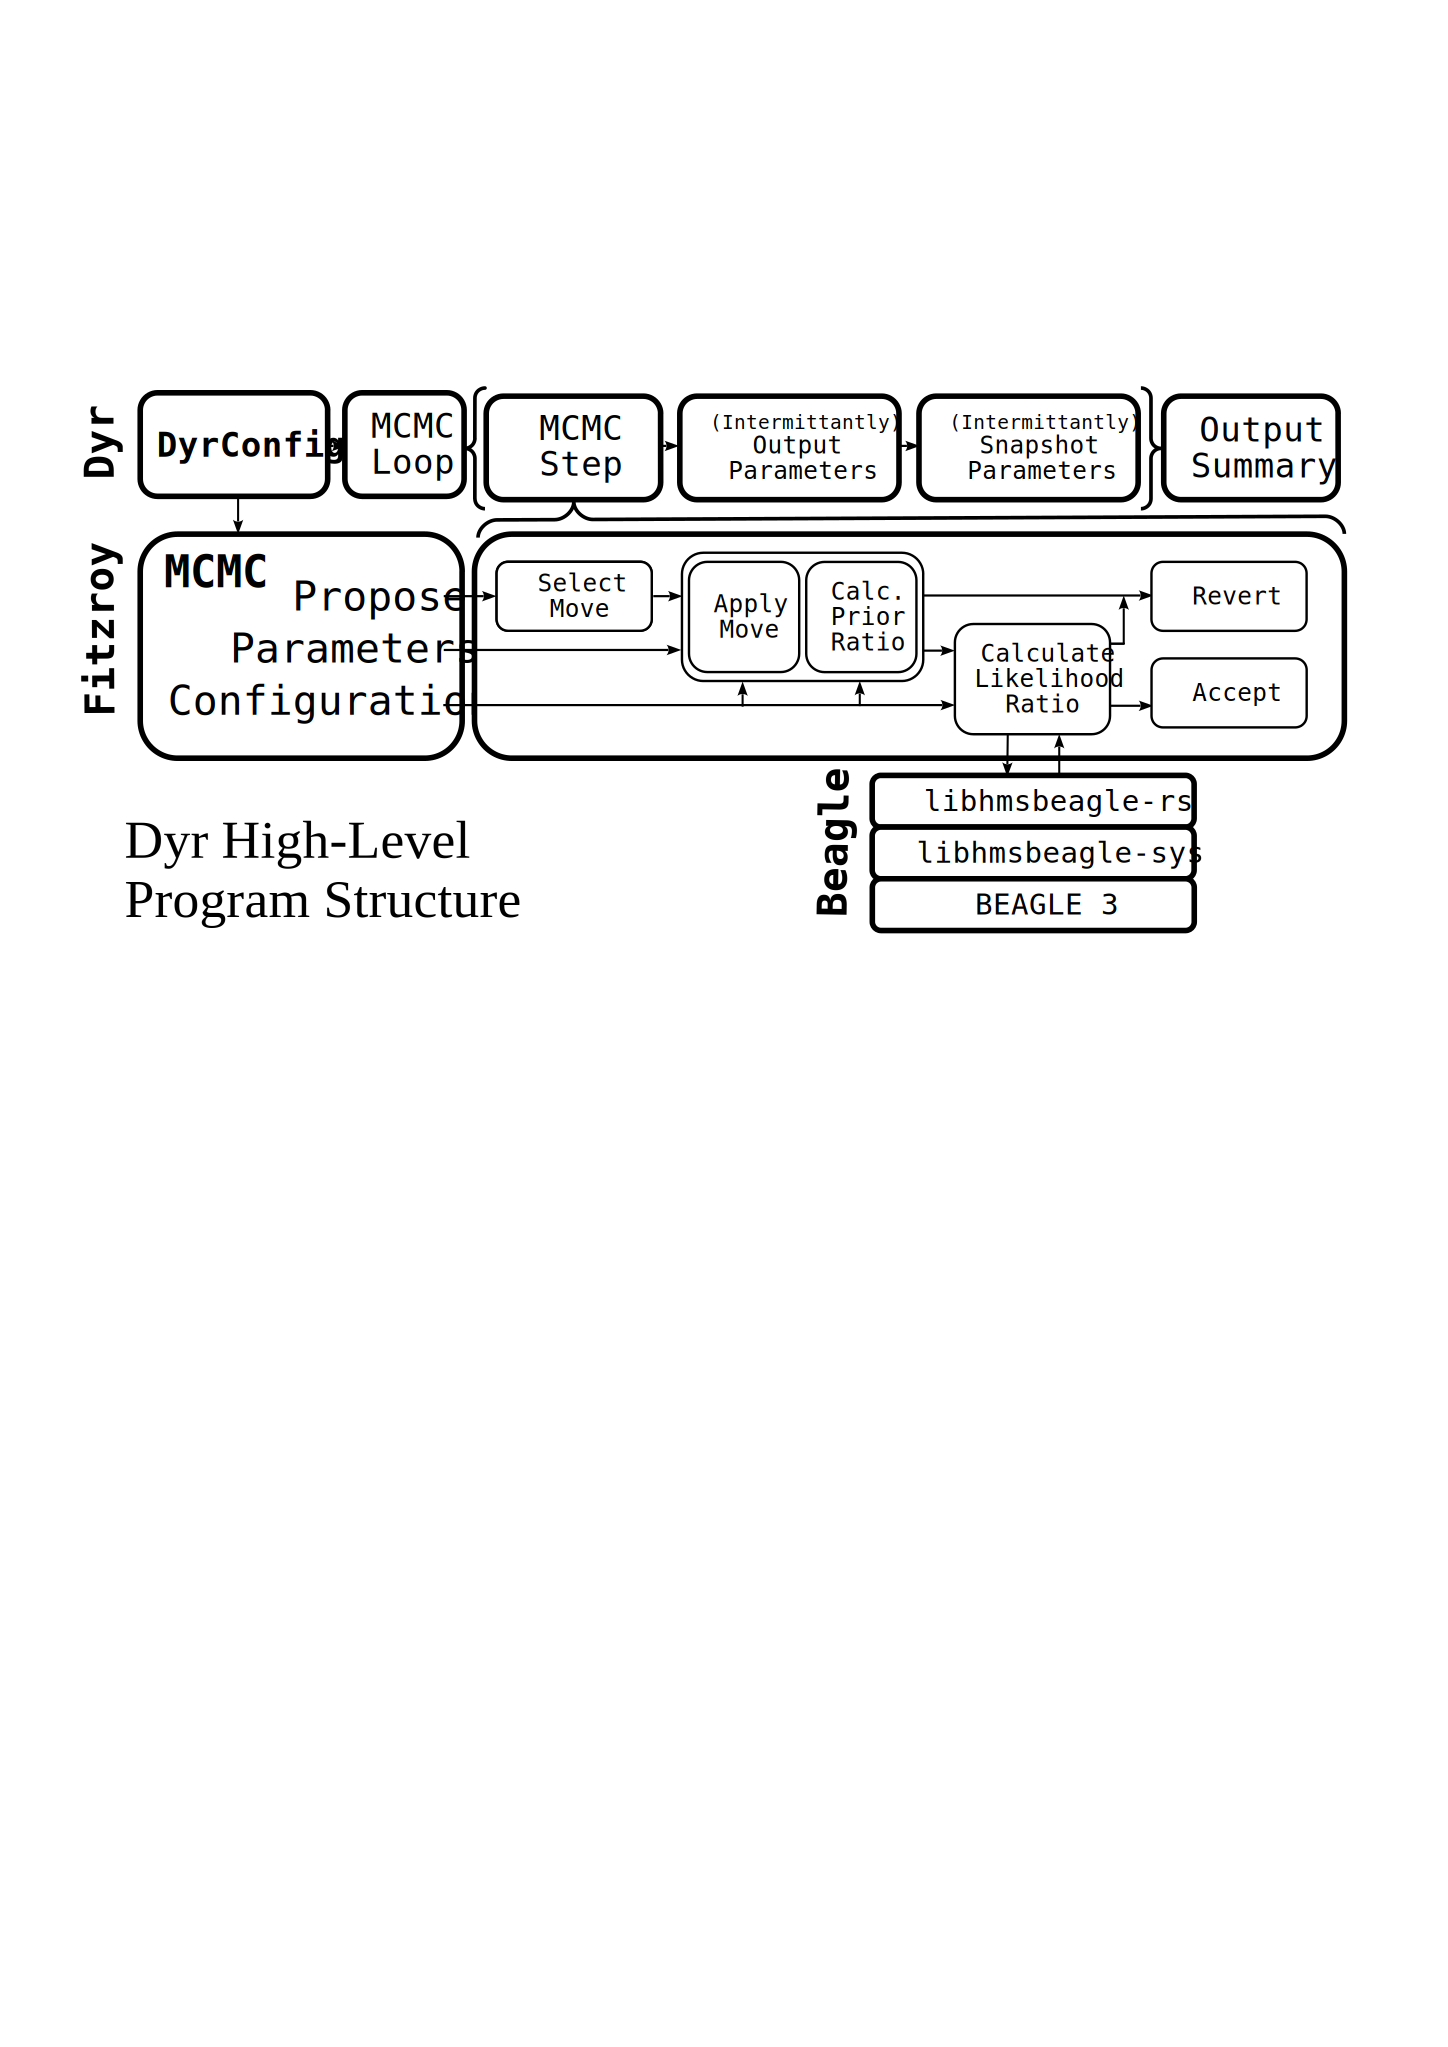
\includegraphics[width=9cm,center]{progdiagram}
\end{figure}

When \textit{Dyr} runs, the first order-of-duty is to build a \texttt{DyrConfig} structure which encodes all the information necessary to perform an inference run. This is then used to instantiate a \texttt{fitzroy::MCMC} structure, which is composed of three key parts: the \texttt{Configuration}, which describes the immutable `scaffold' of the parameter space; the mutable \texttt{Parameters}, which are equivalent to $\Gamma$ in our methodological discussion; and the structure \texttt{Propose}, which manages the proposal distribution. The initial \texttt{Parameters} are drawn at random; care is taken to ensure they have non-zero prior likelihood, but otherwise no attempt is made to choose `good' parameters.

Before starting the Markov Chain, \textit{Dyr} also creates a blank \texttt{fitzroy::Summary} structure, which will serve as a database for intermittently snapshotted phylogenies once the burn-in period of the chain has elapsed. 

The program now enters the main-loop of the Metropolis-Hastings algorithm, which is handled by the  \textit{Dyr} front-end directly. The core logic of the algorithm is wholly contained within the \texttt{step} function of the \texttt{fitzroy::MCMC} instance, and calling this function constitutes the entirity of most iterations. However, at regular intervals, configurable in the manifest, the program outputs information about the current chain state. Furthermore, as previously mentioned, in the latter part of the inference process \textit{Dyr} also takes phylogeny snapshots. These snapshots are only taken once every $1000$ steps to minimise autocorrelation.

At the end of the inference process a Maximum Clade Crediblity (MCC) tree $\psi_{mcc}$ is calculated from the set of snapshotted trees, and output in Newick format.

The topology $\tau_{mcc}$ of the tree $\psi_{mcc}$ is defined as being equal to that of the tree within the set that has the highest sum clade frequency across all its clades, where clade frequency is the number of times a given clade appears within the sample. Then, to calculate the chronology $\delta_{mcc}$ of the MCC tree, we assign each clade root (i.e. node) a date equal to the median date of that clade in the set of trees, and calculate the branch lengths by simply traversing the tree.\footnote{Astute readers will note that this could lead to negative branch lengths. This is considered an acceptable, though unlikely, outcome of the MCC algorithm.}

As it happens, our implementation of Maximum Clade Credibility kills two birds with one stone. Decomposing a tree into a list of its clades, each \texttt{Clade} uniquely identified by a hashable bitstring, is necessary not only for tallying clade frequencies, but also for checking clade and ancestry constraints in the tree prior.

\subsection{A Step in the Chain}

We now take a deeper look at the \texttt{step} function of the Fitzroy MCMC implementation. This function constitutes the heart of the entire system, since its role is to perform a step of the Metropolis-Hastings algorithm.

\subsubsection{Making a Move}

The first task is to draw a new parameterisation from the proposal distribution of the current parameterisation. Up til now we have only spoken abstractly about this as an augmentation of the parameterisation, but in practice the augmenetation is achieved by the selection and application of a `Move' from a set of available `Moves', whereby each Move corresponds to a specific type of modification that can be made to the parameterisation. For example, we have a move called \texttt{TreeNodeSwap}, which chooses two nodes of the tree at random and swaps their attachment points.

The selection and application of a Move is achieved with \texttt{make\_move}, an associated function of \texttt{Propose}. This structure was supplied with the \texttt{Configuration} of the inference run when it was created and therefore only choses from the set of Moves applicable to this run. For example, the move \texttt{CoalescentIntervalResize} is not relevant when there is only one generalised interval (i.e. the population is constant), so in such cases it is not registered in the set of moves at instantiation.

The function \texttt{Propose::make\_move} choses a Move at random (according to a set of hand-tuned weights). In Rust terms, each Move is in fact a structure implementing the trait \texttt{Move}.\footnote{A Rust trait is equivalent to a typeclass in Haskell, and analogous, though not equivalent, to the concept of an abstract superclass in OOP languages.} Each such Move is required to have a function itself called \texttt{make\_move}. This function draws a specific augmentation from its own internal distribution, applies it to the \texttt{Parameters}, calculates the prior likelihood change and the Hastings ratio and returns them.

At this point is is worth noting that although up until now we have spoken about likelihood calculations in the conventional way, internally our software works with the natural logarithms of likelihoods, known as `log-likelihoods'. This is necessary to maintain fidelity when working with the sort of very low likelihoods that are a natural consequence of using distributions over such a large parameter space, and also has the convenient upside of reducing multiplications and divisions into additions and subtractions.

To be precise, every implementation of the function \texttt{Move::make\_move} is required to accept an immutable reference to the \texttt{Configuration} and a mutable reference to the current \texttt{Parameters}, and return a \texttt{MoveResult}, the definition of which is given below.\footnote{Actually, this isn't the real definition; I removed some Rust idiosyncracies.}

\begin{verbatim}
struct MoveResult {
    log_prior_likelihood_delta: double,
    log_hastings_ratio: double,
    revert: Revert,
    damage: Damage
}
\end{verbatim}

The \texttt{log\_prior\_likelihood\_delta} is the change in log prior likelihood, which is the log-likelihood equivalent to the prior likelihood ratio. Similarly, the \texttt{log\_hastings\_ratio} is the log-likelihood equivalent of the Hastings ratio.

\subsubsection{Accept or Reject}

The \texttt{step} function accepts the returned \texttt{MoveResult} and calls a function to calculate the new log marginal likelihood. It then determines the acceptance probability. In log-likelihood terms, this is calculated by summing the log prior likelihood delta, the log marginal likelihood delta, and the log hastings ratio. The augmentation is then accepted if and only if the log acceptance probability is larger than the log of a uniform random variable in the range $[0, 1]$.

If the move is not accepted then we need to revert the state of the \texttt{Parameters} back to their previous state. We have devised an elegant and flexible method for achieving this. In the definition of \texttt{MoveResult} above, note that there is a field \texttt{revert} of type \texttt{Revert}. The type \texttt{Revert} is a heap-allocated closure (anonymous function) that accepts the current state of the MCMC chain as a mutable reference. Each Move constructs a closure that closes upon (embeds) the stored previous state of whichever parameter the Move augmented. If the \texttt{step} function decides to revert the Move, all it needs to do to restore the old state of the \texttt{Parameters} is call the closure \texttt{revert()}.

This approach is elegant and efficient. It is elegant because the step function needs to know nothing at all about any of the individual Moves; it is perfectly generic. Furthermore, the usage of a closure to encapsulate the cached state means that the Move object itself can be entirely stateless. Moreover, it is efficient because the closure only stores the \texttt{Parameters} that have changed. If a Move simply alters a global rate parameter, then the tree itself remains unmodified and therefore its state does not need to be cached. If state caching was performed within the \texttt{step} function itself, its lack of knowledge about the specific move that had been made would require it to clone the entire set of \texttt{Parameters}, at considerable cost to both computational and memory resources. 

If the move is accepted, the \texttt{revert} closure is never called. In any case, after having accepted or rejected the proposed parameterisation, the \texttt{step} function concludes: one iteration of Metropolis-Hastings has been completed.


\subsubsection{Marginal Likelihood}
  
Although it is easily the most computationally intensive part of the inference process, we have only so far touched upon the calculation of log marginal likelihood. As discussed, the low-level heavy-lifting is performed by the BEAGLE 3 library. However, making this library usable and ergonomic in Rust requires three abstraction layers. 

The first is the raw Rust bindings to the BEAGLE C API. These are auto-generated by the Rust library `bindgen'. The second is the low-level wrapper interface. This interface still exposes essentially the same functions as are present in the BEAGLE API, but it provides a translation layer between Rust types and C types. For example, the C type \texttt{*double}, a potentially null 64-bit float pointer, corresponds to the Rust type \texttt{Option<\&mut f64>} -- an algebraic type that can optionally store a mutable reference to 64-bit float. These two layers together constitute \texttt{libhmsbeagle-sys} -- a safe and usable, though unidiomatic, Rust binding to BEAGLE.

The third abstraction layer is provided by \texttt{libhmsbeagle-rs}, which consumes the interface provided by \texttt{libhmsbeagle-sys}, and in turn exposes a powerful and idiomatic Rust reimagining of BEAGLE's core interface.

Its first idiomaticisation is to wrap BEAGLE's instance API in an RAII\footnote{Resource Allocation Is Initialisation} \texttt{Instance} structure. This means that for as long as an \texttt{Instance} is allocated in memory, it corresponds to a valid and live instance within BEAGLE.

However, the most powerful abstraction that the \texttt{Instance} structure provides is what we refer to as 'buffer alternates'. To understand this feature, we must first consider the two basic datastructures upon which BEAGLE operates: partial likelihood buffers, or 'partials' for short; and transition matrix buffers, or simply 'matrices'. Every internal node of the phylogeny requires a corresponding partials buffer, while every node except for the root requires a corresponding transition matrix.

When 'buffer alternates' are enabled, our system allocates two partials for each internal node and two matrices for each node excepting the root. These are known as `main' and `alternate' buffers. For each pair of buffers, we maintain a boolean flag in a structure called \texttt{Alternates} which signals which of the main and alternates buffer is currently active. Therefore, when we update a node's matrix, or re-calculate its partials, we take care to do so exclusively using the active buffers.

To demonstrate what the benefit is of all this additional book-keeping, we must explain the purpose of the final parameter of the \texttt{MoveResult} structure, \texttt{damage}. Each Move is obliged to create a \texttt{Damage} object, which records the matrices and partials which have been invalidated by its augmentation to the \texttt{Parameters}.

As an aside, if any partial is invalidated, all partials between it and the root are necessarily also invalidated, so the \texttt{Damage} structure has an associated function \texttt{mark\_partials\_to\_root} to make this particular form of invalidation easier to inscribe.

When a Move has been made, the \texttt{step} function calls another function called \texttt{flip\_by\_damage}, which switches all the partials and matrices which have been `damaged' (i.e. invalidated) onto their other buffer, be that the main or the alternate.

Having flipped the appropriate buffers, the \texttt{step} function is free to calculate the new log marginal likelihood. Again using the \texttt{Damage} as a reference, an array of new likelihood operations is constructed and passed to BEAGLE. Each operation corresponds to a single step of Felsenstein's algorithm; involving only a node and its two children. This ensures that no more than the minimum amount of computation necessary to compute the new log marginal likelihood is performed.

The operations are applied, the new log marginal likelihood is summed and read-off from the root node, and control flow returns to the \texttt{step} function, as we have seen. Now the purpose of the whole enterprise becomes apparent: in the instance that the augmentation is rejected, the \texttt{flip\_by\_damage} function is called again with the same \texttt{Damage} as an argument, and the effective state of the BEAGLE likelihood engine \texttt{Instance} is as if the new parameterisation had never been suggested. Conversely, if the new parameterisation is accepted, the buffers are not flipped again; they become themselves the baseline state of the system.

It may not be immediately obvious why this is such a key optimisation until one considers that an MCMC process might reject many successive moves. Without buffer alternates, which enable a baseline state of the likelihood engine to be preserved until the chain advances, each rejected move would require a ground-up likelihood recalculation.

\subsection{Implementing Rate Variation}

We previously described the evolutionary rates at each branch, for each site, in equation \eqref{eqn:rate}. However, that description abstracted over the practical implementation, which although essentially equivalent in outcome, follows a somewhat non-obvious methodology.

\subsubsection{Among Site Rate Variation}

As stated, we consider site rates to be drawn from a Gamma distribution with mean $1$, described by a shape parameter $\alpha$. However, it would be computationally infeasible to actually seelct a different site rate from this Gamma distribution for each site. Therefore, we instead use a standard technique, known as the `Discrete Gamma Model'. In this approach, we slice our site-rate Gamma distribution into $k$ categories, each with equal probability mass, and then take the mean of each category. The likelihood of the data evolving along an edge is therefore taken to be equal to the the average  likelihood across each of the Gamma category rates. Conventionally, $4$ such Gamma categories are used, which is considered to be sufficient to produce a good approximation.

It may not be immediately obvious why this approach is equivalent to selecting specific Gamma site rates from a prior distribution. To understand why this approach is effective, one should recall that MCMC is essentially an method for approximating the integral of the posterior likelihood function. In esssence, then, the Discrete Gamma Model simply approximates the integration step for the site-rate parameters directly. As mentioned, the main reason for this is computational cost. By using a Discrete Gamma Model with $k$ site-rate categories, we multiply the computational cost of performing Felsenstein's algorithm by $k$. This is still somewhat painful, even with $k=4$, but it is much more tolerable than the far greater cost that would be endured if each site had a separate rate, inferred through MCMC.

\subsubsection{Among Branch Rate Variation}

In a similar manner to site-rates, we model branch-rates as being drawn from a distribution with mean $1$, and with shape parameter $\beta$. A key difference, though, is that here the distribution is Log-Normal. Additionally, since each branch likelihood calculation is performed separately, there is no significant computational cost to inferring different rates for each branch. As with site-rates, our approach begins with splitting up the Log-Normal distribution into categories. Our approach here is to construct as many categories as there are branches. As with our site-rate categories, each has equal probability mass. We then assign each branch a category index. For example, the branch with category $0$ has branch-rate equal to the mean of the left-most Log-Normal category, the branch with category $1$ has branch-rate equal to the mean of the second left-most category, and so on up until the right-most category, which is category $n - 1$,assuming the tree has $n$ branches. The purpose of this indirection is to allow us to modify the shape parameter $\beta$ by an MCMC move without invalidating the category assignment. As shall be discussed, we also have an MCMC move to swap rate categories between branches.

BEAGLE allows us to set the value of a given transition matrix based on a model (i.e. the rate matrix and the site-rate categories) and an edge length. When we provide the edge lengths, what we actually provide is the branch length multiplied by the base rate multiplied by the branch-rate corresponding to that branch's rate allocation. In this way the transition matrices are prepared for usage in likelihood calculations.

\subsection{Decomposing the Rate Matrix}

An expression for the rate matrix \textbf{Q} is given in equation \eqref{eqn:ratematrix}. For BEAGLE to use this rate matrix in its likelihood calculations it requires us to provide it in decomposed form, as eigenvalues, eigenvectors, and inverse eigenvectors.\footnote{The columns of the inverse of the matrix of eigenvectors} We need multiply through by the scale factor outside the matrix:

\begin{equation}
    \textbf{Q} = \begin{bmatrix}
-a & a\\
b & -b
\end{bmatrix} \text{ \ given that \ } a = \frac{1}{2 \pi_0} \;,\; b = \frac{1}{2 \pi_1}
\end{equation}

\noindent Then the eigen decomposition of \textbf{Q} is the following:
\begin{align*}
    \text{Eigenvectors} &= [1,\, 1],\;\;  [-\frac{a}{b},\, 1] \\
    \text{Inverse Eigenvectors} &= [\pi_0,\, -\pi_0],\;\;  [\pi_1,\, \pi_0]\\
    \text{Eigenvalues} &= 0,\;\; -a-b
\end{align*}

This is the decomposed form of the rate matrix that is used by BEAGLE. Its simplicity is a pleasant consequence of our relatively simple Binary GTR model; for more complicated rate matrixes, performing this decomposition can be substantially harder.

\subsection{Spanning the Parameter Space}

An important implementation practicality of MCMC is ensuring that the algorithm is able to efficiently move about the parameter space, and (in principle) be able to reach every non-zero prior likelihood parameterisation. This is achieved by choosing an sufficiently broad set of MCMC moves. Our proposal distribution supports the following moves:

\subsubsection{Tree LOCAL Move}

The most complex move we implement, the LOCAL move was outlined by Larget and Simon in a 1999 paper. We present a brief outline of this operation.

First, an edge between internal nodes, $(v, u)$, is selected, such that $v$ is the parent of $u$. We will discuss only the general case where $v$ is not the root; a modified, though fundamentally similar procedure is followed if $v$ is the root. Therefore $v$ has a parent node which we call $w$. Between them, $v$ and $u$ have three additional children. We will refer to the children of $u$ as $a$ and $b$, and the child of $v$ that is not $u$ as $c$ (see Fig. \ref{fig:local}).

Our intention is to randomly assign new heights to the nodes $v$ and $u$, and re-attach their children $a$, $b$, and $c$ at random. So, for example, $c$, which starts out as the child of $v$, may be re-attached as a child of $u$.

However, we observe that there are four constraints on the new heights that we give to $v$ and $u$. Firstly, neither $v$ nor $u$ can be moved higher than $w$. Secondly, $u$ must not be moved higher than $v$. And thirdly, to allow us to re-attach all three children, $u$ must remain above at least two of $a$, $b$, and $c$, while $v$ must remain above all three. Note that in some cases it may be possible for $v$ to move below one of $a$ and $b$, so long as it remains above the other and also remains above $c$.

Therefore, to implement the LOCAL move, we create two uniform distributions and draw a value from each. The first distribution is between the height of $w$, and the height of the highest node out of $a$, $b$, and $c$. We call the value we draw from this distribution $h_1$. The second distribution is between the height of $w$, and the height of the second highest node out of $a$, $b$, and $c$. We call the value we draw from this distribution $h_2$.

It is probable, though not certain, that $h_1 > h_2$. However what is certain is that both values are higher than the lowest two child nodes, and at least one of them is higher than the highest child node. So we can safely use these values as the new heights of $v$, and $u$. Naturally, we use the higher value out of $h_1$ and $h_2$ as the new height of $v$, and the lower of the two as the new height of $u$.

We now re-attach $a$, $b$, and $c$. If $h_2$ happened to be lower than the highest child node, then we have no choice in the matter. In this case it is certain that $h_2$ is lower than $h_1$, and therefore is the new height of $u$, and therefore $u$ is lower than the highest child node. So the highest child node is attached to $v$, and the lower two are attached to $u$.

Conversely, if $h_2$ is higher than the highest child node, then we can re-attach the children any way we like. We choose one node out of $a$, $b$, and $c$ at random to be the child of $v$, and the other two become the children of $u$.

Re-attaching the children is the final step of the LOCAL move. The genius of it is that since it only modifies one small section of the tree, it does not require any fiddly and computationally expensive recursions to propogate changes across the entire structure. The nodes that form the 'perimeter' of the focused segment -- namely $w$, $a$, $b$, and $c$ -- are fixed in place; all that changes is $v$ and $u$, and the edges linking $v$ and $u$ to the rest of the tree. Nonetheless, since it allows nodes to change parents, as well as change height, the LOCAL move alone is capable of almost entirely spanning the space of possible trees. In fact, the only desirable augmentation to the tree the LOCAL move is not capable of making is changing the dates of tips, since they can never be either $u$ or $v$. For achieving that, we need a separate move.

One important consideration when implementing the LOCAL move is the Hastings Ratio. This needs to be taken into account in cases where the node $u$ moves `across' the level of $c$. When $u$ moves from from below the level of $c$ to above it, any of the three child nodes can be chosen to attach to $v$. However, if we consider the same move in reverse, with $u$ moving from above the level of $c$ to below it, there is only one possible outcome, which is for the child nodes to remain attached as they were before. Therefore, the same move has three times the likelihood density in the proposal distribution going backwards when compared to going forwards. To account for this, the Hastings Ratio for the forwards move is $3$, while it is $\frac{1}{3}$ for the backwards move. 
\begin{figure}
\caption{An example of a tree segment as seen by the LOCAL move}\label{fig:local}
\vspace{0.2cm}
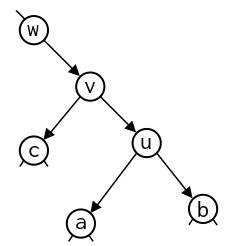
\includegraphics[width=4cm,center]{local}
\end{figure}

\subsubsection{Tree Tip Move}
As mentioned, the only thing the LOCAL move is unable to do to augment our trees is modify tip (leaf) ages. For most tips this is not a problem, as most tips are fixed in the present day ($t = 0$). However, as mentioned previously, our software supports a type of constraint called a tip calibration, which allows a tip to fall anywhere within a specified date range. These calibrations are of outsize importance for our project, since they are essentially the `yardstick' by which time-depth is determined. We therefore implement a move which nudges the position of a randomly chosen tip-calibrated taxa by a small, random amount.

\subsubsection{Tree Node Swap}
The LOCAL move and the tip move are sufficient to fully span the space of possible trees. However, to improve convergence, escape local minima, and prevent constraints from `trapping' the tree in specific regions of parameter space, we implement a third tree operation. The tree node swap is as it sounds; we choose two nodes and attempt to swap them. If it is impossible to do so (for example, if one node is younger than the other's parent), then we consider the move to have zero prior density and abort. Since we deal with log-likelihoods, we handle this case by returning from \texttt{make\_move} a log prior likelhood delta of $-\infty$. This is handled as a special case in the \texttt{step} function and results in instant rejection, short-circuiting the marginal likelihood calculation. Several moves use this facility when they select augmentations that they find to be \textit{a priori} impossible.

\subsubsection{Coalescent Interval Resize}

This move applies only when the generalised skyline tree prior is in use. This move selects a generalised interval and resizes it. Recall that a generalised interval is a contiguous grouping of coalescent intervals. Therefore, this move can be conceived of as taking a coalescent interval from the beginning or end of one generalised interval, and giving it to the adjacent generalised interval. Of course, care is taken to ensure that a generalised interval is never left with zero width.

\subsubsection{Coalescent Population Rescale and Augment}

There are two moves for augmenting the coalescent population parameters. The rescale move multiplies all the paramaters by the same randomly chosen factor, while the augment move multiples a single randomly chosen parameter by a randomly chosen factor. In principle, the augment move alone could span the parameter space, however the rescale move is also implemented to improve convergence and to allow the tree prior to `respond' to changes in timescale.

\subsubsection{ABRV Category Swap}

As has been discussed, each branch is assigned the index of a branch-rate category. This move selects two branches at random and swaps their indices. This move produces no change in prior likelihood, since branch-rates are considered uncorrelated, and has no Hastings ratio. Therefore its success or failure is wholly dependant on the marginal likelihood ratio (and, of course, random chance).

\subsubsection{ABRV Shape, ASRV Shape, and Base Rate}

Each of these rate-related parameters has an associated MCMC move. In each case, a narrow Normal distribution around the current value is used to propose the new value for the parameter. It is not necessary to calculate Hastings ratios, since the Normal distribution is symmetric, however it is important to catch the case of the selected value being less than or equal to zero and assign it zero prior density. As discussed, each of these paramaters has its own prior distribution; thus we duly calculate the change in log prior density in each case.

\subsubsection{Pi One Move}

The final move is the $\pi_1$ move. Recall that $\pi_1$, the stationary frequency of trait-presence, may vary between $0$ and $1$. It has a uniform prior, so excepting cases where the proposed value -- again drawn from a narrow Normal distribution -- is out-of-bounds, there is no change in log prior likelihood. As with all global substitution model parameters, changing this value causes `full damage' to the tree and thus all transition matrices and prior buffers must be recalculated.

\section{Results and Analysis}\label{sec:results}

We now show the results of applying \textit{Dyr} to real datasets. We use the same curated \textsc{Narrow}, \textsc{Medium}, and \textsc{Broad} subsets of the IELEX Indo-European lexical trait database as Chang et al. and Rama.

We first present our main analyses, using our preferred prior model -- the constant-population coalescent prior with clade and ancestry constraints.

\begin{center}
    \begin{tabular}{ |c|c|c| }
    \hline
    Analysis&Dataset&Root Age\\
    \hline
    A&\textsc{Broad}&6008\\
    B&\textsc{Medium}&7692\\
    C&\textsc{Narrow}&6309\\
    \hline
    \end{tabular}
\end{center}

Analysis A, which uses the \textsc{Broad} dataset, yields an MCC tree with a root age of 6008 years before present. This root age firmly supports the Steppe hypothesis for the origin of Proto-Indo-European, which is premised on a root age of between 5500 and 6500 years before the present.

Analysis B, which uses the \textsc{Medium} dataset, yields an MCC tree with a root age of 7692 years before present. This root age is harder to intepret, being too old for the standard window of the Steppe hypothesis, but too young for that of the Anatolian hypothesis (between 8000 and 9500 years before present). Our results here are in line with those of Chang et al. and Rama, who both find that the \textsc{Medium} dataset yields substantially older root ages than either the \textsc{Broad} or \textsc{Narrow} datasets.

Analysis C, which uses the \textsc{Narrow} dataset, yields an MCC tree with a root age of 6309 years before present. As with the \textsc{Broad} dataset, this root age is firmly in the domain of the Steppe hypothesis. This analysis is of particular interest as it is directly comparable to analysis A6 of Chang et al., which yielded a root age of 6130 years before present. Clearly these dates are similar, and inspires confidence that our software is functioning correctly. However, they are not the same -- why is this? One reason might be that Chang et al. implement a feature called `ascertainment bias correction', which aims to account for postulated traits which are not observed at any tips. Another reason is of course simply the randomness inherent to any finite stochastic process -- though this should be fairly minimal in the long, highly converged chains that both our analyses used. Finally, the possibility of course exists that subtle bugs or differences in how our software implements various parts of the MCMC process have affected the results. If this is the case, though, the impact does not seem to be too dramatic.

To further investigate the correlation between the results of our software and those obtained by Chang et. al, we tried to replicate their analysis A3, which employs the \textsc{Broad} dataset and the generalised skyline plot tree prior with $5$ generalised intervals. Their analysis yielded a root age of 5950 before present, while ours was just slightly older at 6022 -- not significantly different from our equivalent result with the constant-population prior, in fact. This result furthers our confidence in the reliability of \textit{Dyr} and in its capability on real-world phylolinguistic tasks.

Of course, it is not sufficient for our software to simply produce `good numbers'. As we have sermonised throughout this paper, it is also paramount that the results of an analysis be consistent with linguistic realities. Happily, an inspection of our inferred phylogenies reveals that even in unconstrained regions, our analyses are consistent with contemporary linguistic scholarship. For example, the closer relationship of Breton to Cornish than to Welsh is recognised in the phylogenies. Furthermore, Romance subgroups such as the Gallo-Romance (Provencal, Walloon, and French) and Rhaetian languages (Ladin, Romansh, and Friulian) are recognised and form clades in our trees. In general, the inferred MCC trees appear linguistically sound; not only topologically but chronologically; for example the inferred ages of the Latvian-Lithuanian split at between 1000 and 1300 years before present are in close agreement with the academic consenus, which suggests contact with Balto-Finnic and Slavic between the 7th and 10th centuries as an impetus for the schism.\cite{baltic2018}

On balance, we consider our results to be potent -- if not conclusive -- evidence to support the Steppe hypothesis for the Indo-European \textit{Urheimat}, re-affirming the prior results of Chang et al.

\subsection{Convergence}

For an MCMC system to be reliable and efficient, it is important that it consistently reaches the desired stationary distribution from an arbitrary starting point in parameter space. This can be investigated by means of a convergence graph. We present such a graph in Fig. \ref{fig:convergence}, which shows how the log posterior likelihood approaches zero in the early stages (i.e. the `burn-in') of an MCMC run.

The plateaus visible in the convergence graph are not, as one might perhaps expect, the algorithm getting stuck in local minima, but rather instances where the algorithm has not yet `solved' constraints. As has been discussed, constraints are implemented (slightly inelegantly) as large penalties on log prior likelihood. When the MCMC process `solves' a constraint, this penalty is lifted, the effect of which is sufficient to ensure that it is practically impossible for the constraint to ever be broken by a subsequent move.

In Fig. \ref{fig:convtrees}, we present four phylogenies selected from various points in the MCMC run depicted in Fig. \ref{fig:convergence}. Recall that the initial topology of the tree is almost completely random -- the only concession to optimality made is that it is chosen to satisfy tip calibrations, to ensure the phylogeny has non-zero prior likelihood.

In the first phylogeny depicted in Fig. \ref{fig:convtrees}, the algorithm has only taken $9,999$ steps, and it can be seen that it is still very far from optimal, having taken just begun its walk towards the desired stationary distribution. See how the Celtic and Gothic language families are interleaved, and at such oddities as Irish and Romanian appearing mixed in with the Indo-Aryan languages.

In the second tree, at step $19,999$, the algorithm has clearly progressed, and is much closer to having reached a `sensible' topology. However, some glaring erorrs still remain, such as Avestan being more closely related to the Indo-Aryan languages than Vedic Sanskrit, and the Greek and Armenian clades remaining interwoven.

By the third phylogeny, at step $599,999$, the algorithm has solved all-but-one of the constraints, with the only exception being the ancestry constraint on Old Irish. This constraint penalty accounts for the final plateau in the convergence graph. In general, though, this phylogeny is looking quite plausible, with only a few oddities, such as Faroese being grouped closer with Norwegian than Icelandic. This might be a sign that the algorithm is still a little way off convergence, or equally plausibly is simply stochastic noise. The reader may also note the surprisingly old root age of this phylogeny; this too is probably largely a consequence of the randomness inherent to the stochastic process, but perhaps in part is due to the un-solved Celtic clade slowing the evolution rate via the `jogging' effect.

The final snapshot, from step $999,999$, satisfies all constraints, and is a perfectly plausible candidate as an Indo-European phylogeny. We note that the algorithm has properly inferred near-zero length branches for all our specified ancestral taxa. By inspection of this tree, and also by reference to the convergence graph, we can deem this phylogeny to be drawn from the posterior likelihood distribution. At this point, in a full analysis, it would be proper to start taking snapshots from which to build the final MCC tree.

\begin{figure}
\caption{Convergence on constrained \textsc{Narrow} dataset}\label{fig:convergence}
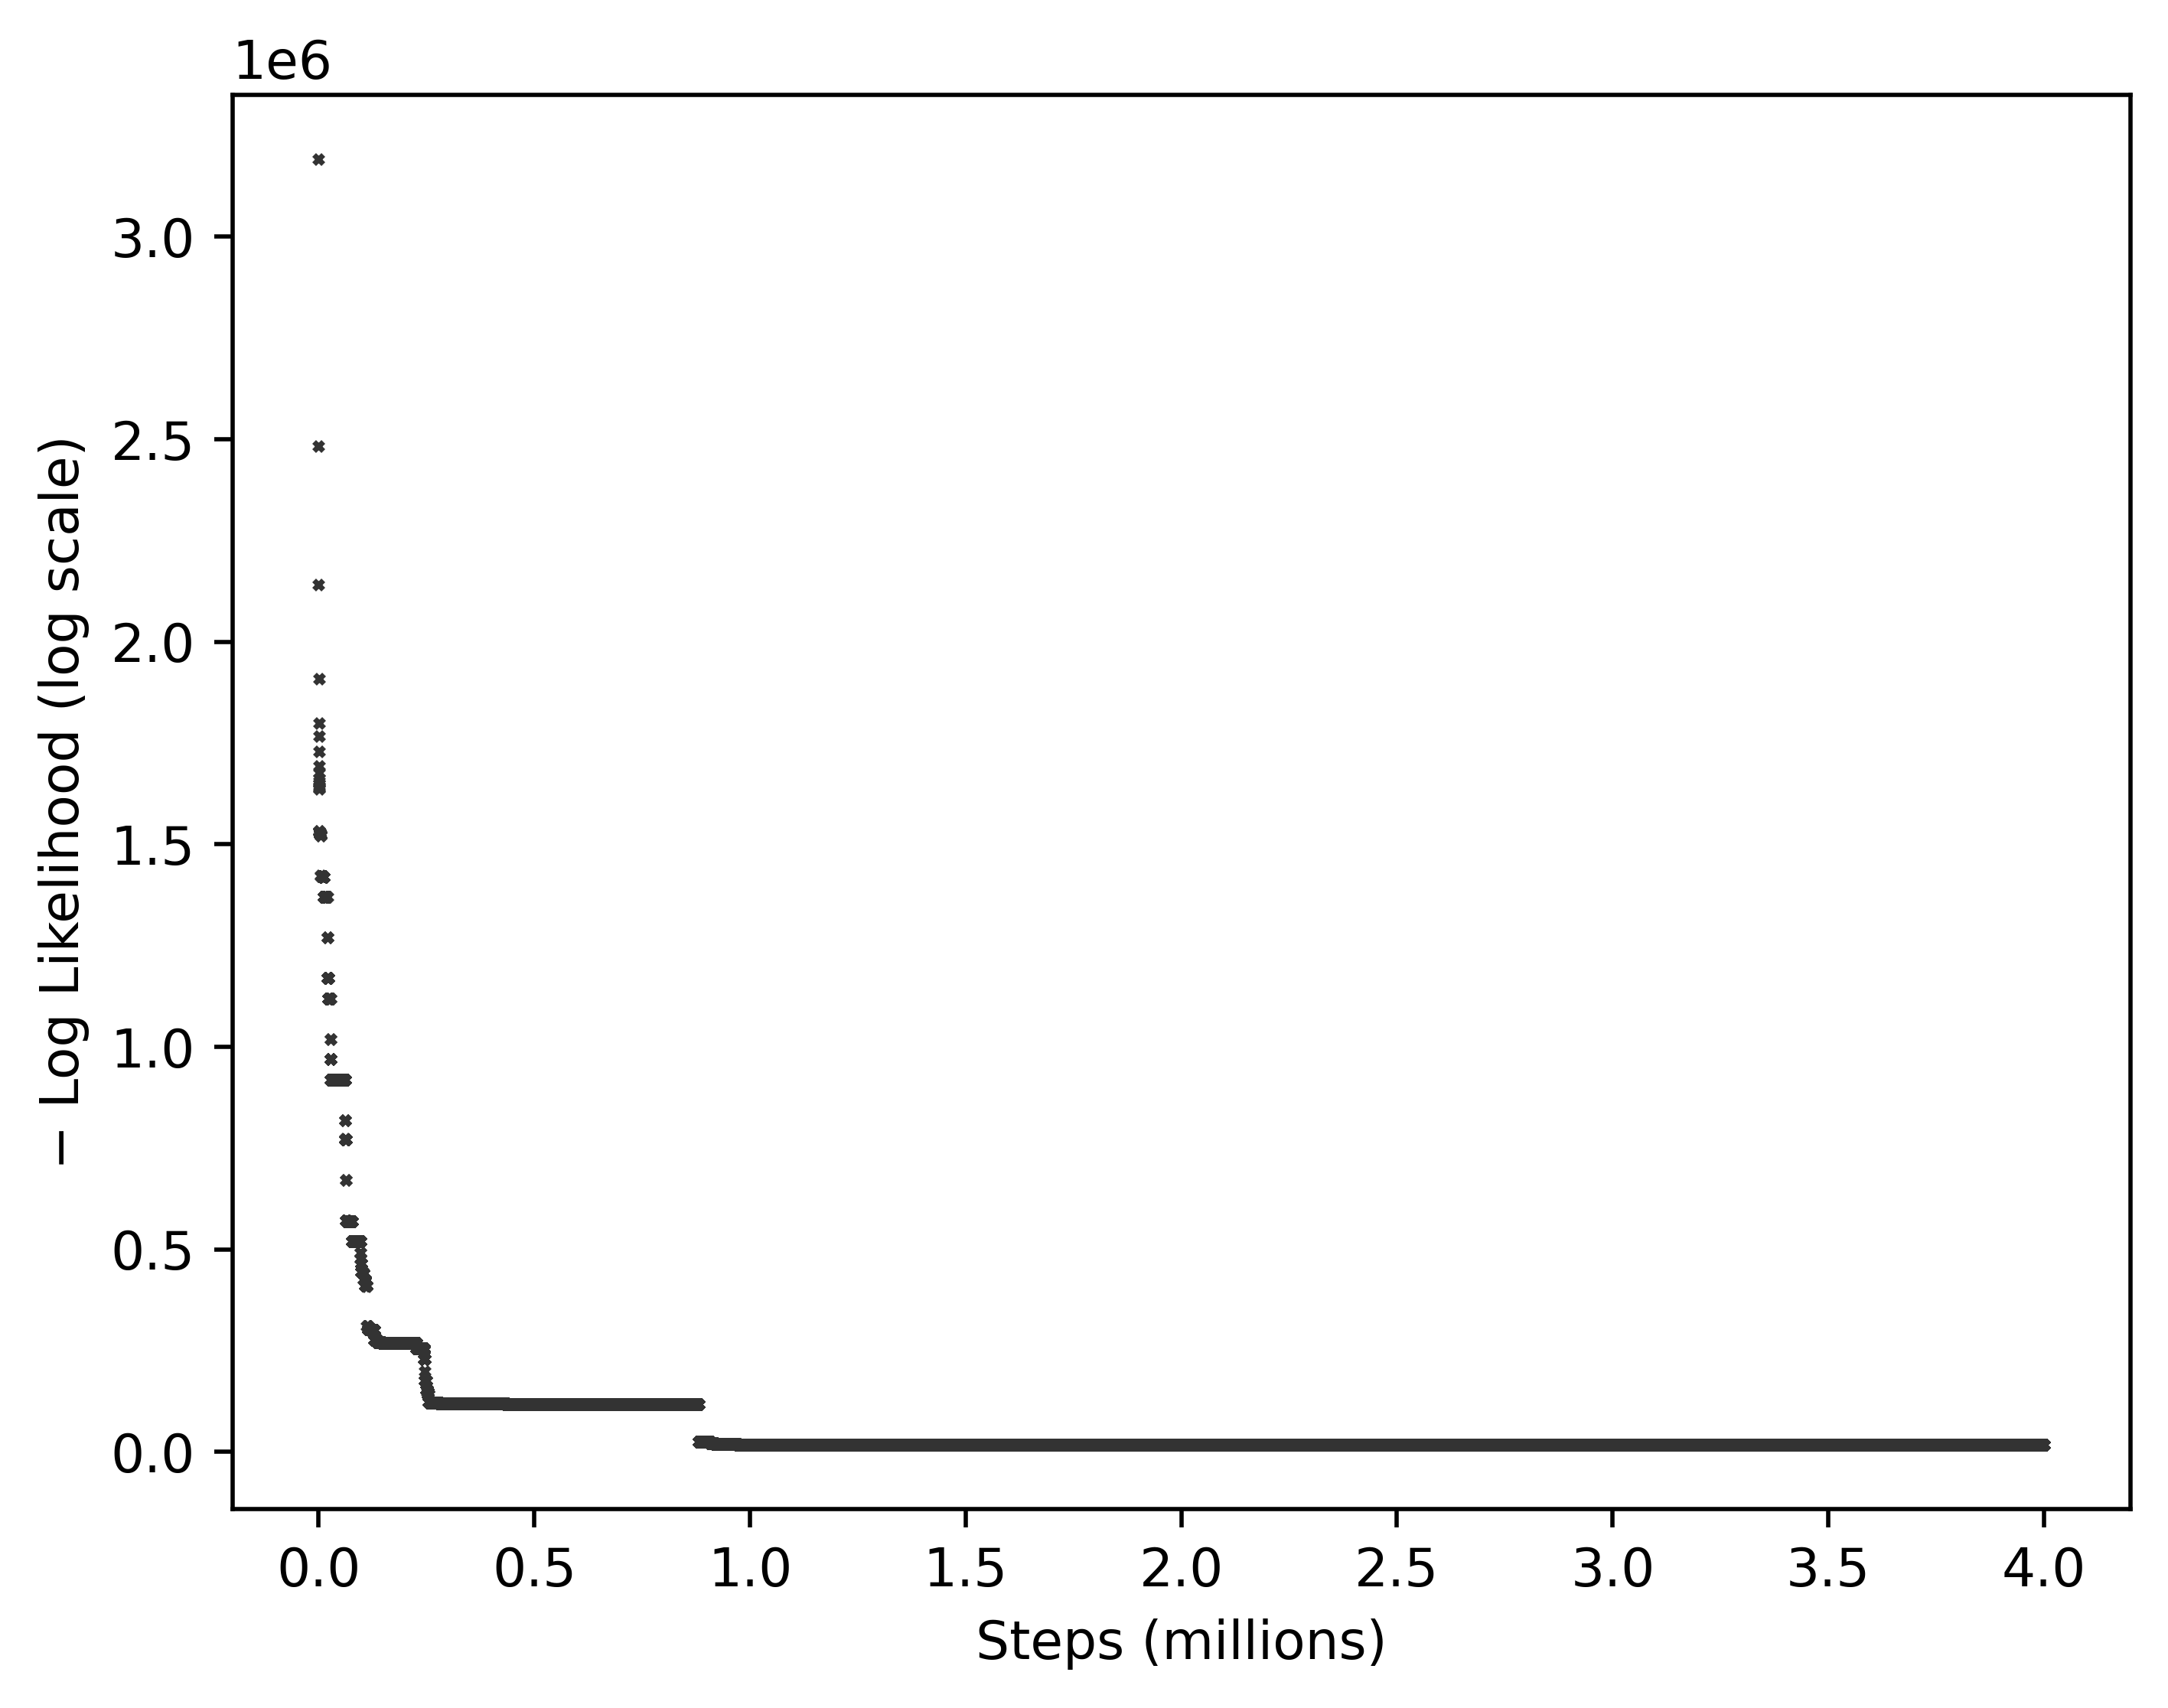
\includegraphics[width=8cm,center]{convergence}
\end{figure}

\begin{figure*}
    \caption{Analysis A: \textsc{Broad}, constant-population coalescent prior, clade+ancestry constraints, 48M steps (MCC tree).}\label{fig:analysisA}
    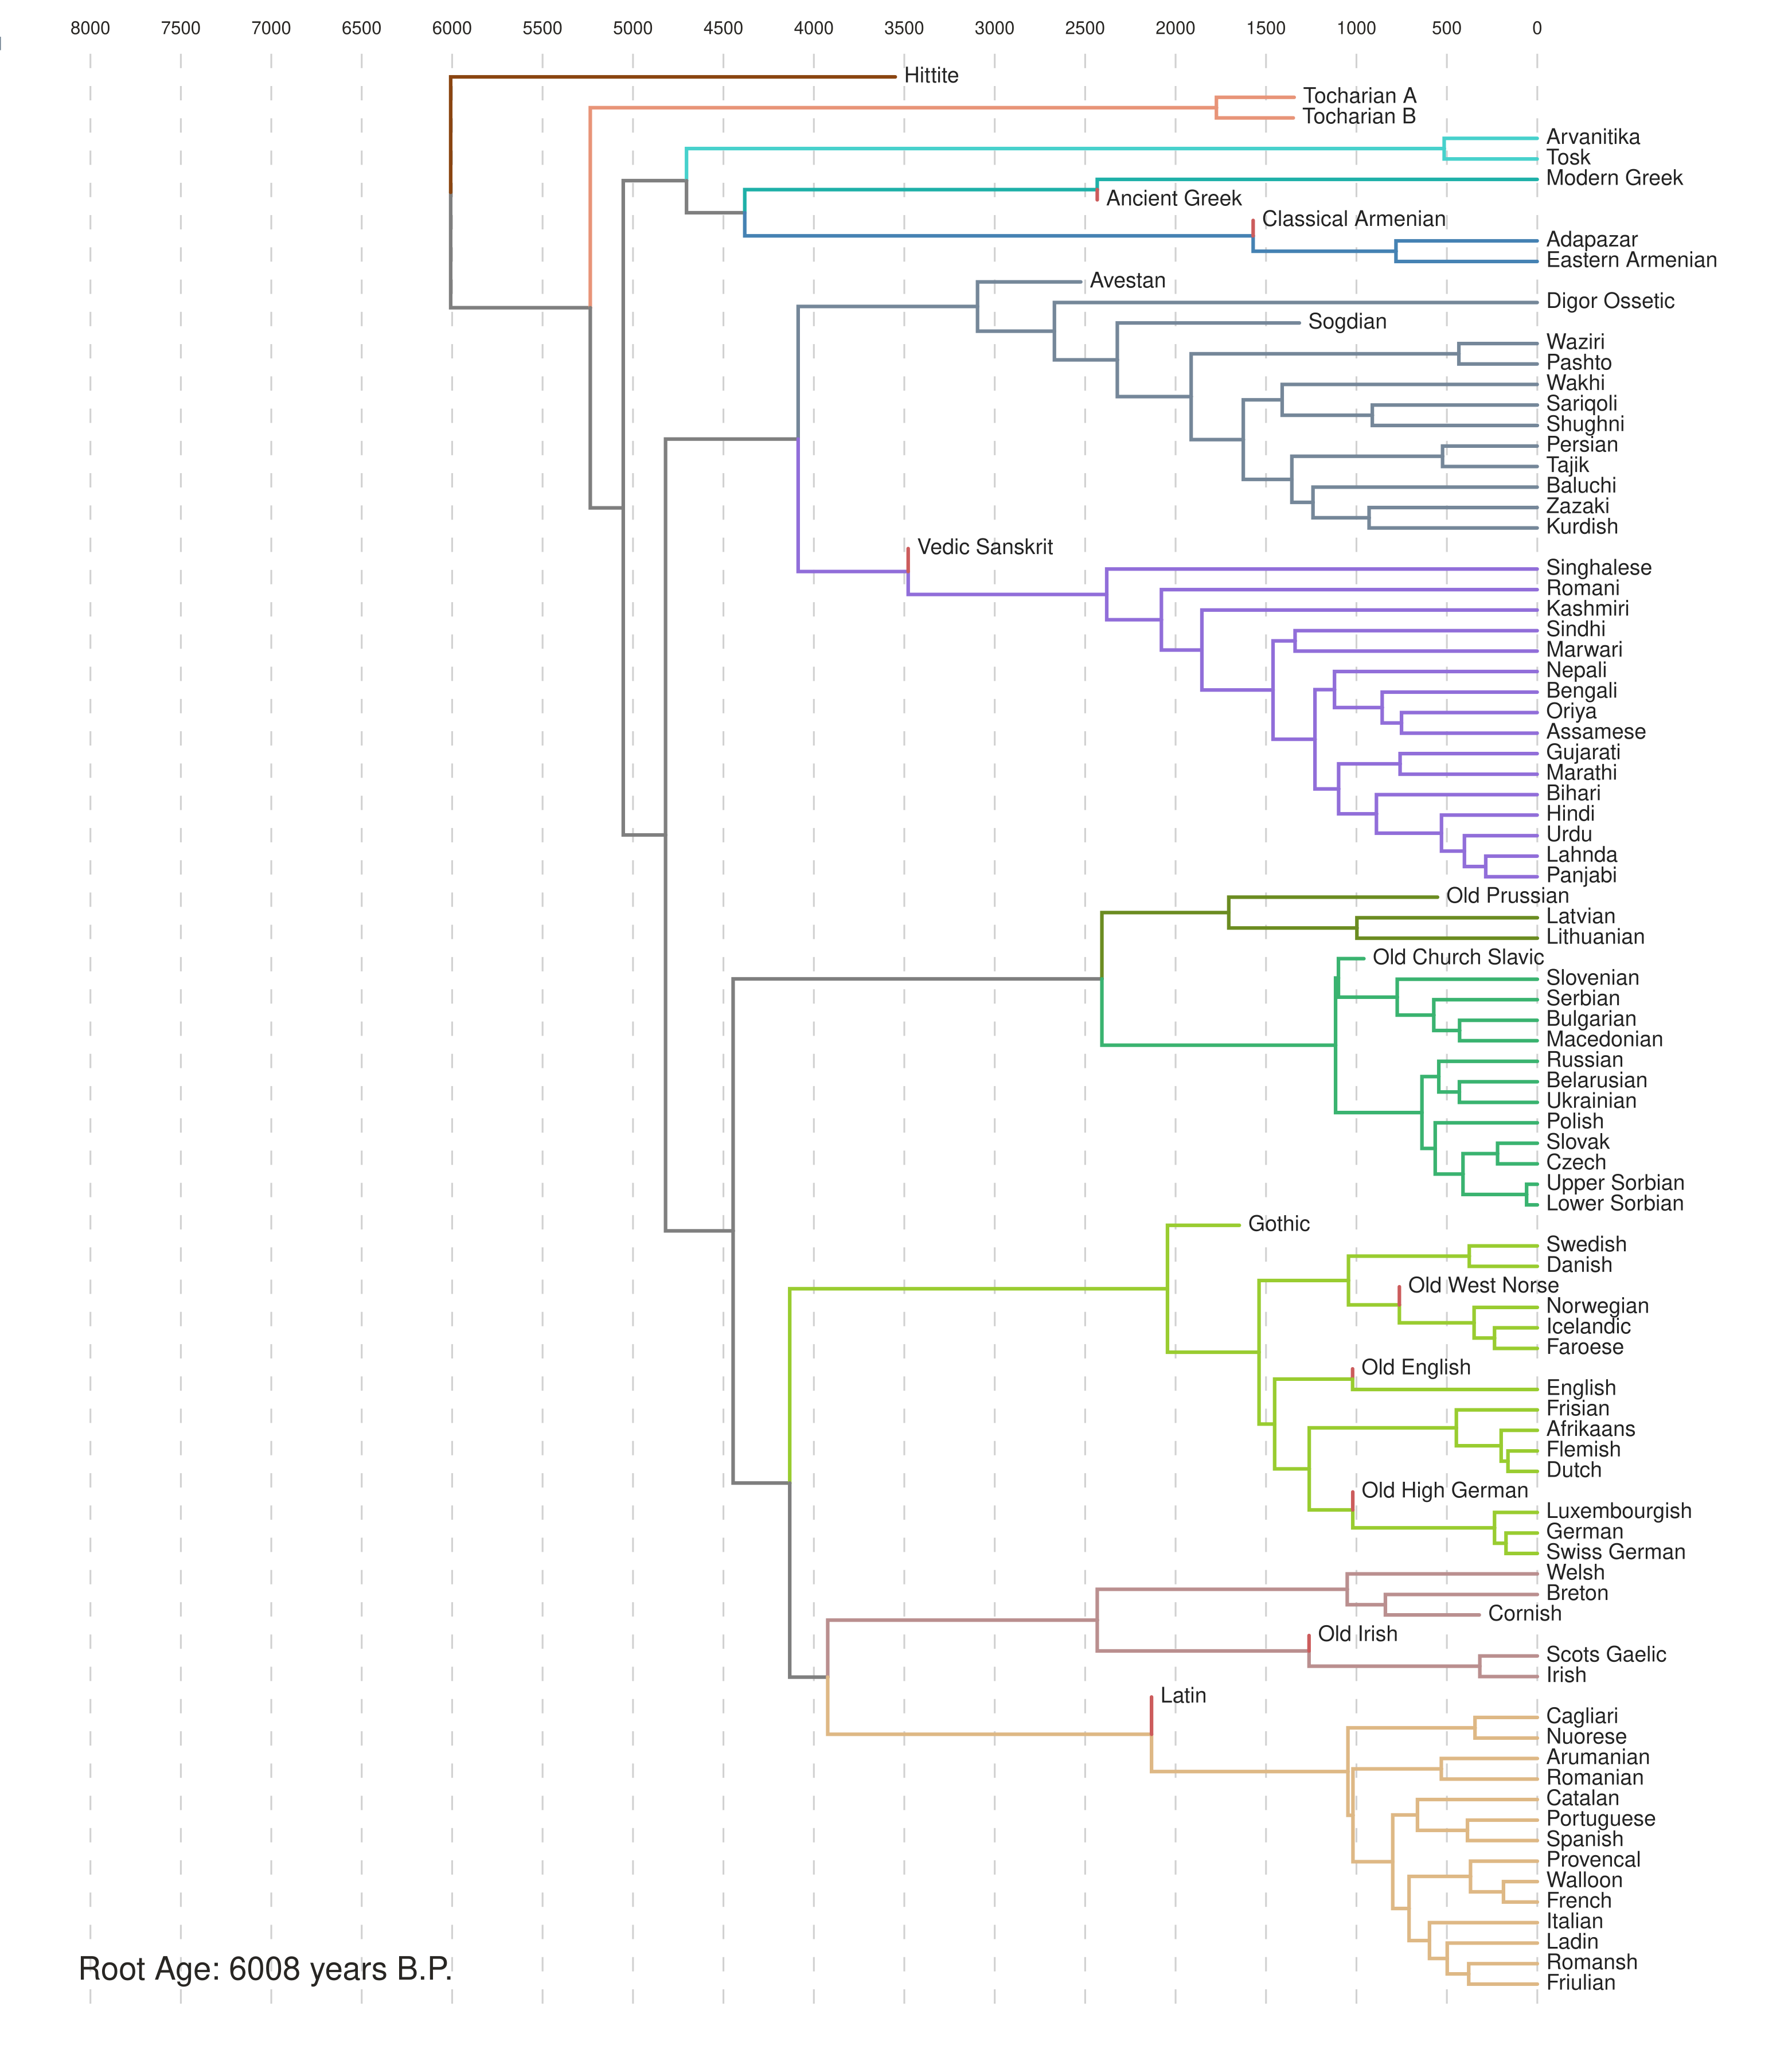
\includegraphics[width=\textwidth, center]{runs24-broad-constant}
\end{figure*}

\begin{figure*}
    \caption{Analysis B: \textsc{Medium}, constant-population coalescent prior, clade+ancestry constraints, 48M steps (MCC tree).}\label{fig:analysisB}
    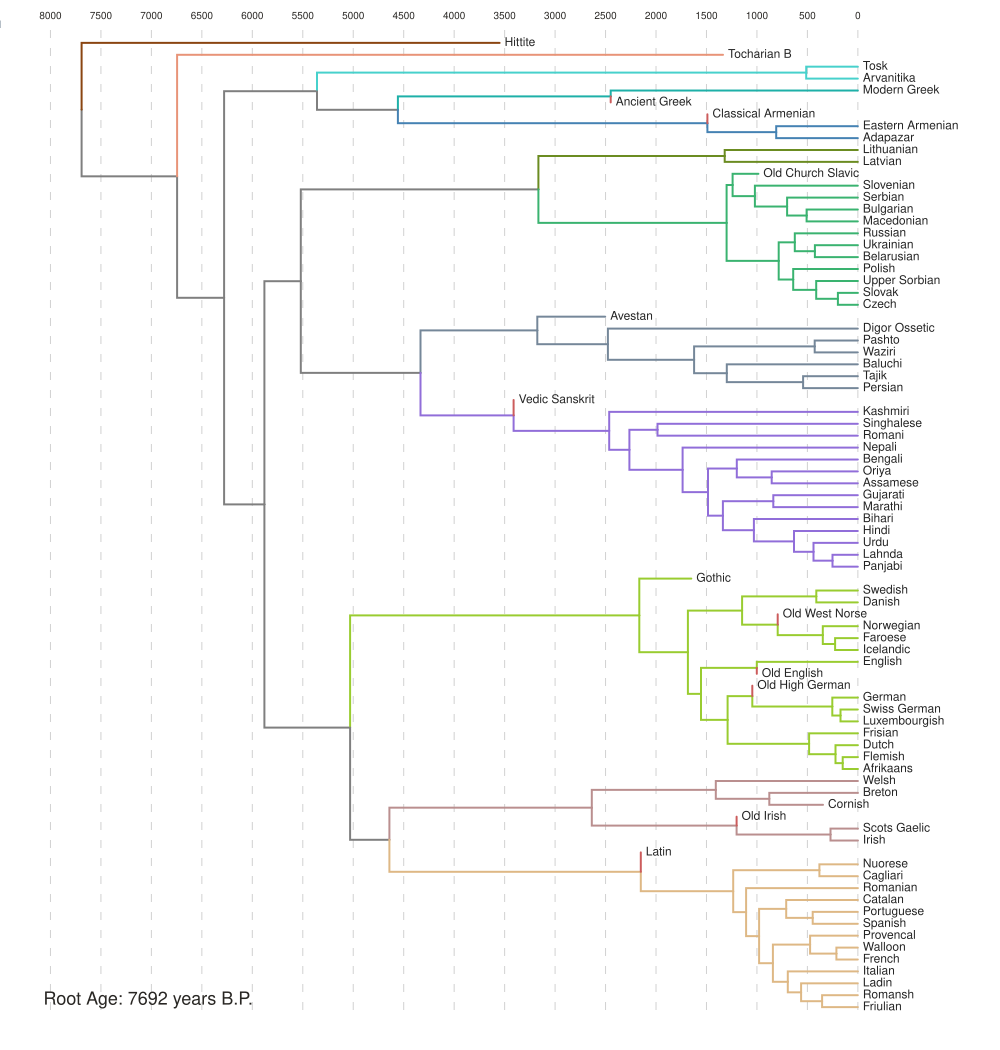
\includegraphics[width=\textwidth, center]{runs24-medium-constant}
\end{figure*}

\begin{figure*}
    \caption{Analysis C: \textsc{Narrow}, constant-population coalescent prior, clade+ancestry constraints, 96M steps (MCC tree).}\label{fig:analysisC}
    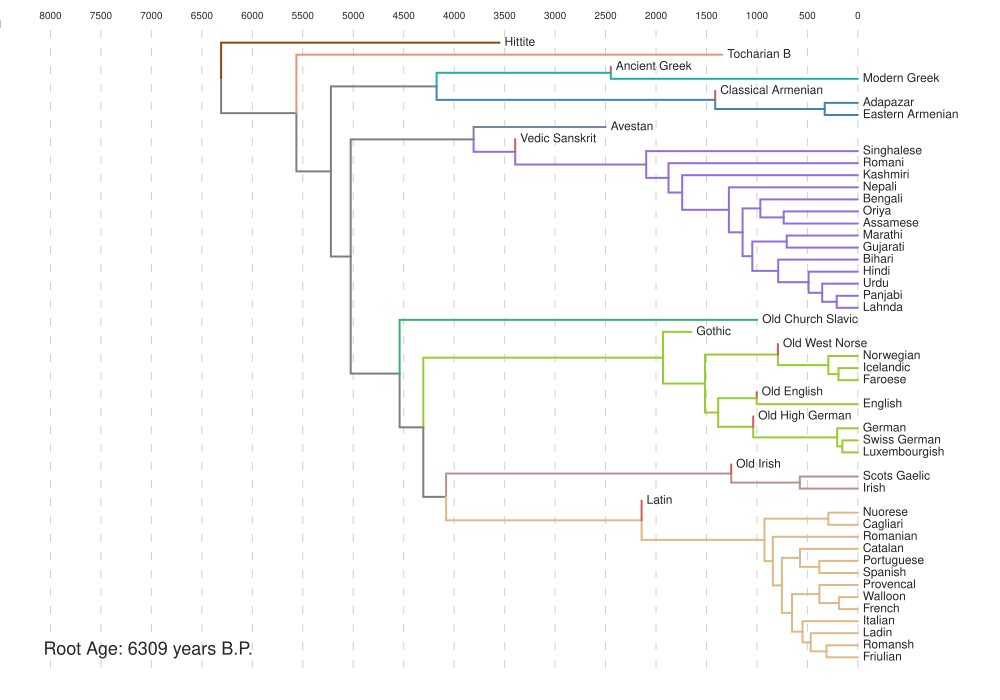
\includegraphics[width=\textwidth, center]{runs24-narrow-constant}
\end{figure*}


%\begin{figure*}
%    \caption{Analysis D: \textsc{Broad}, generalised skyline plot coalescent prior, clade+ancestry %constraints, 48M steps (MCC tree).}\label{fig:analysisD}
%    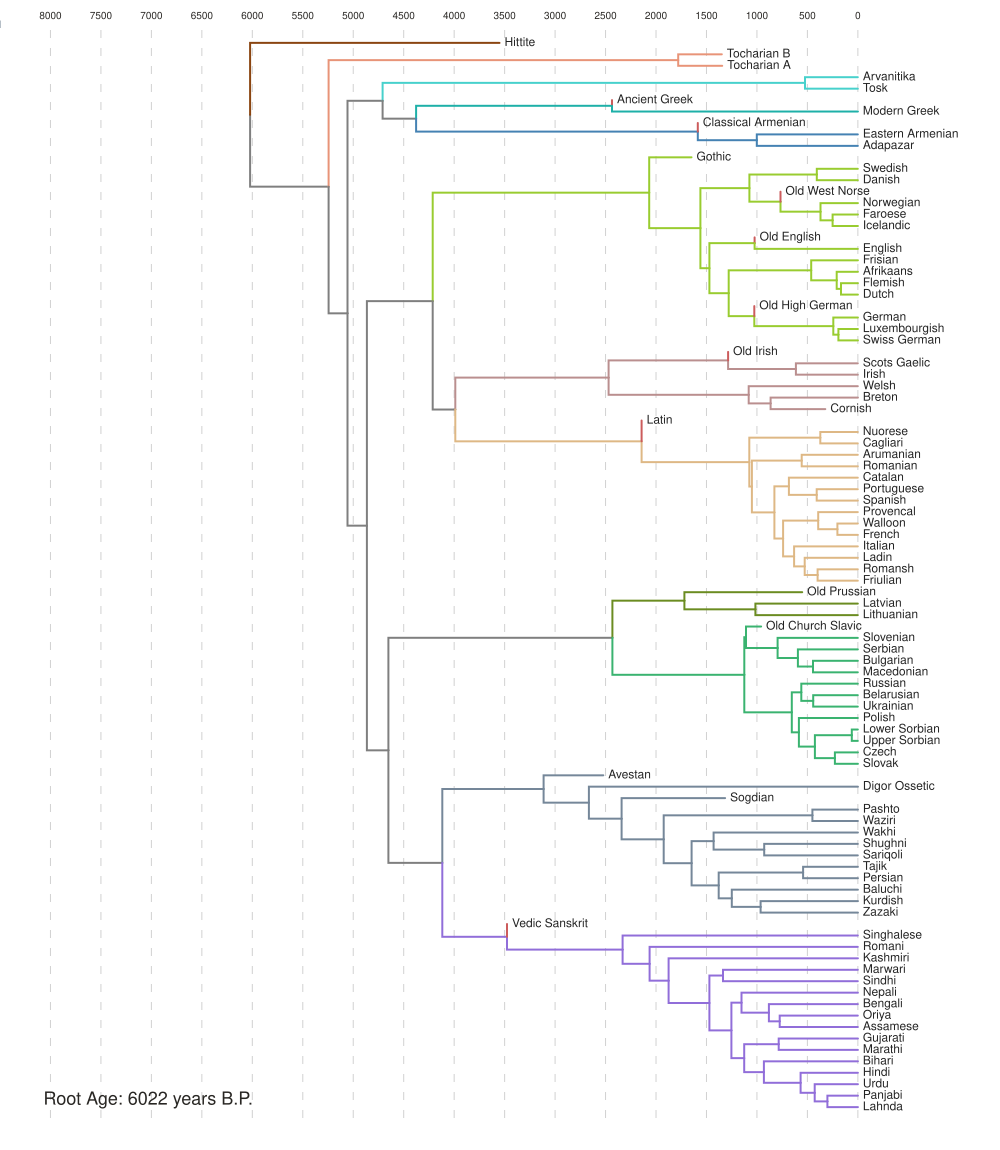
\includegraphics[width=\textwidth, center]{runs24-broad-generalised}
%\end{figure*}


\begin{figure*}
     \centering
     \begin{subfigure}[b]{0.4\paperwidth}
         \centering
         \caption{Phylogeny after 9,999 steps}
         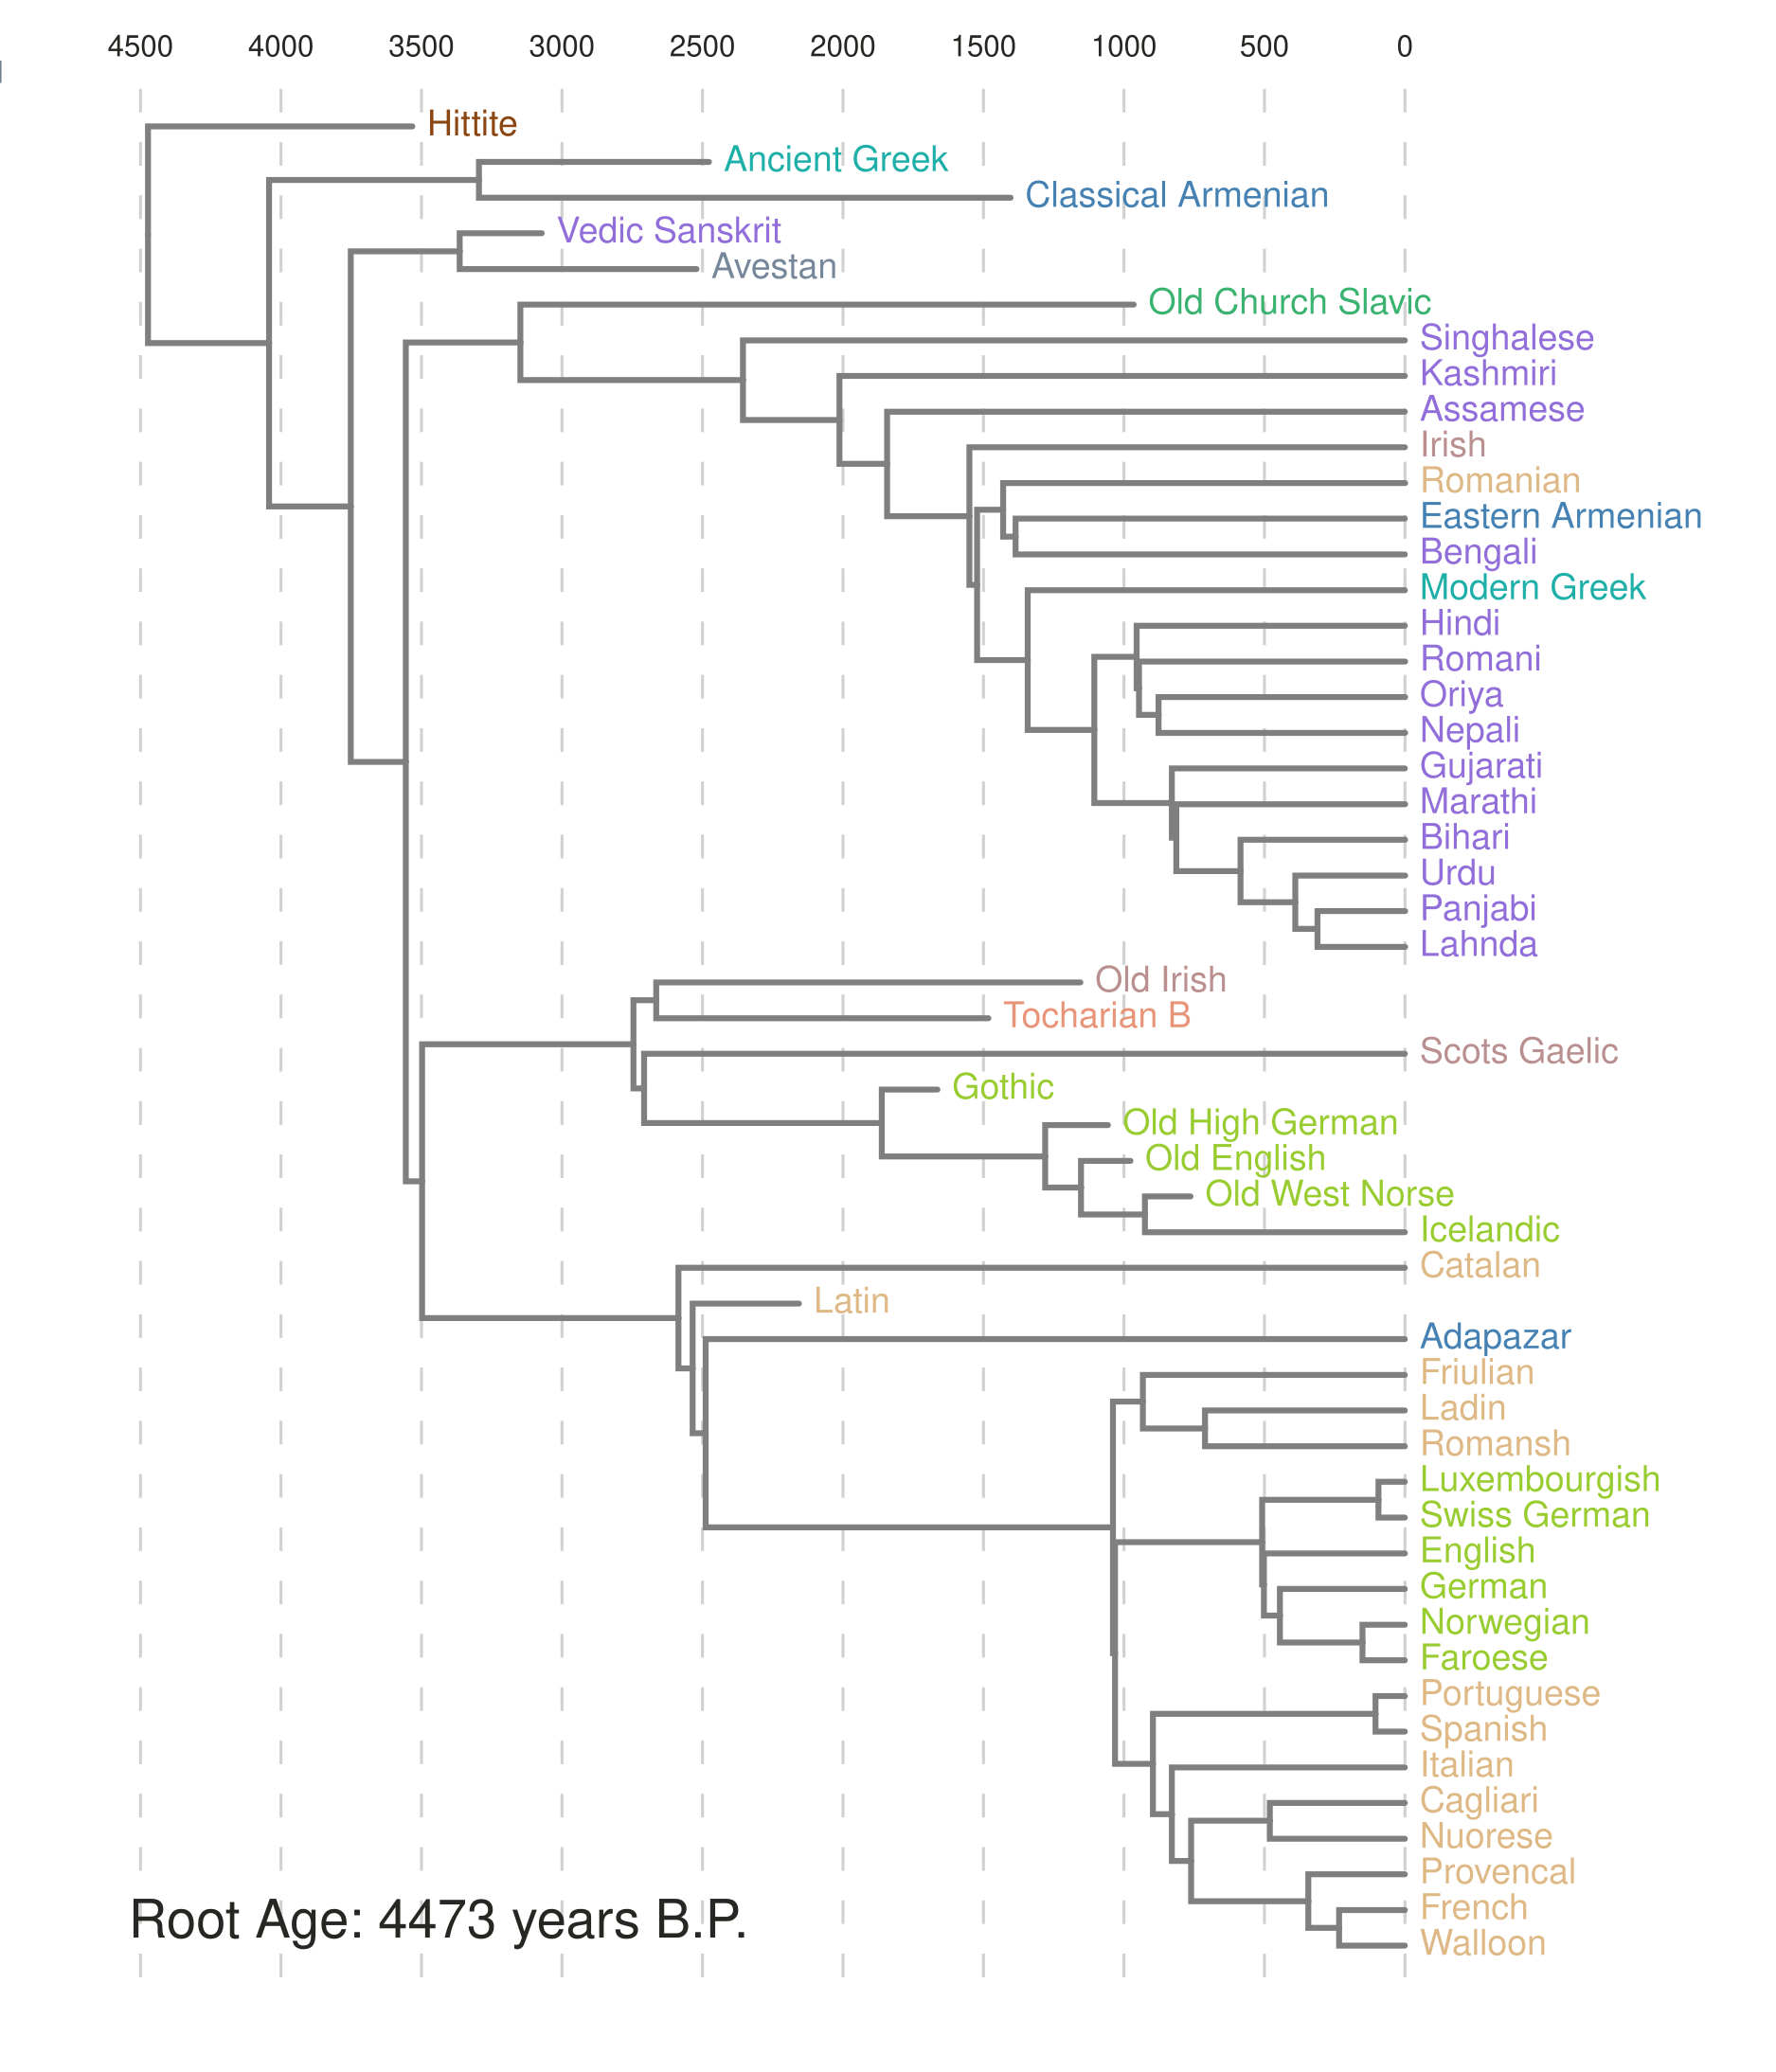
\includegraphics[width=\textwidth]{runs26-conv1}
         \label{fig:convtree1}
     \end{subfigure}
     \hfill
     \begin{subfigure}[b]{0.4\paperwidth}
         \centering
         \caption{Phylogeny after 199,999 steps}
         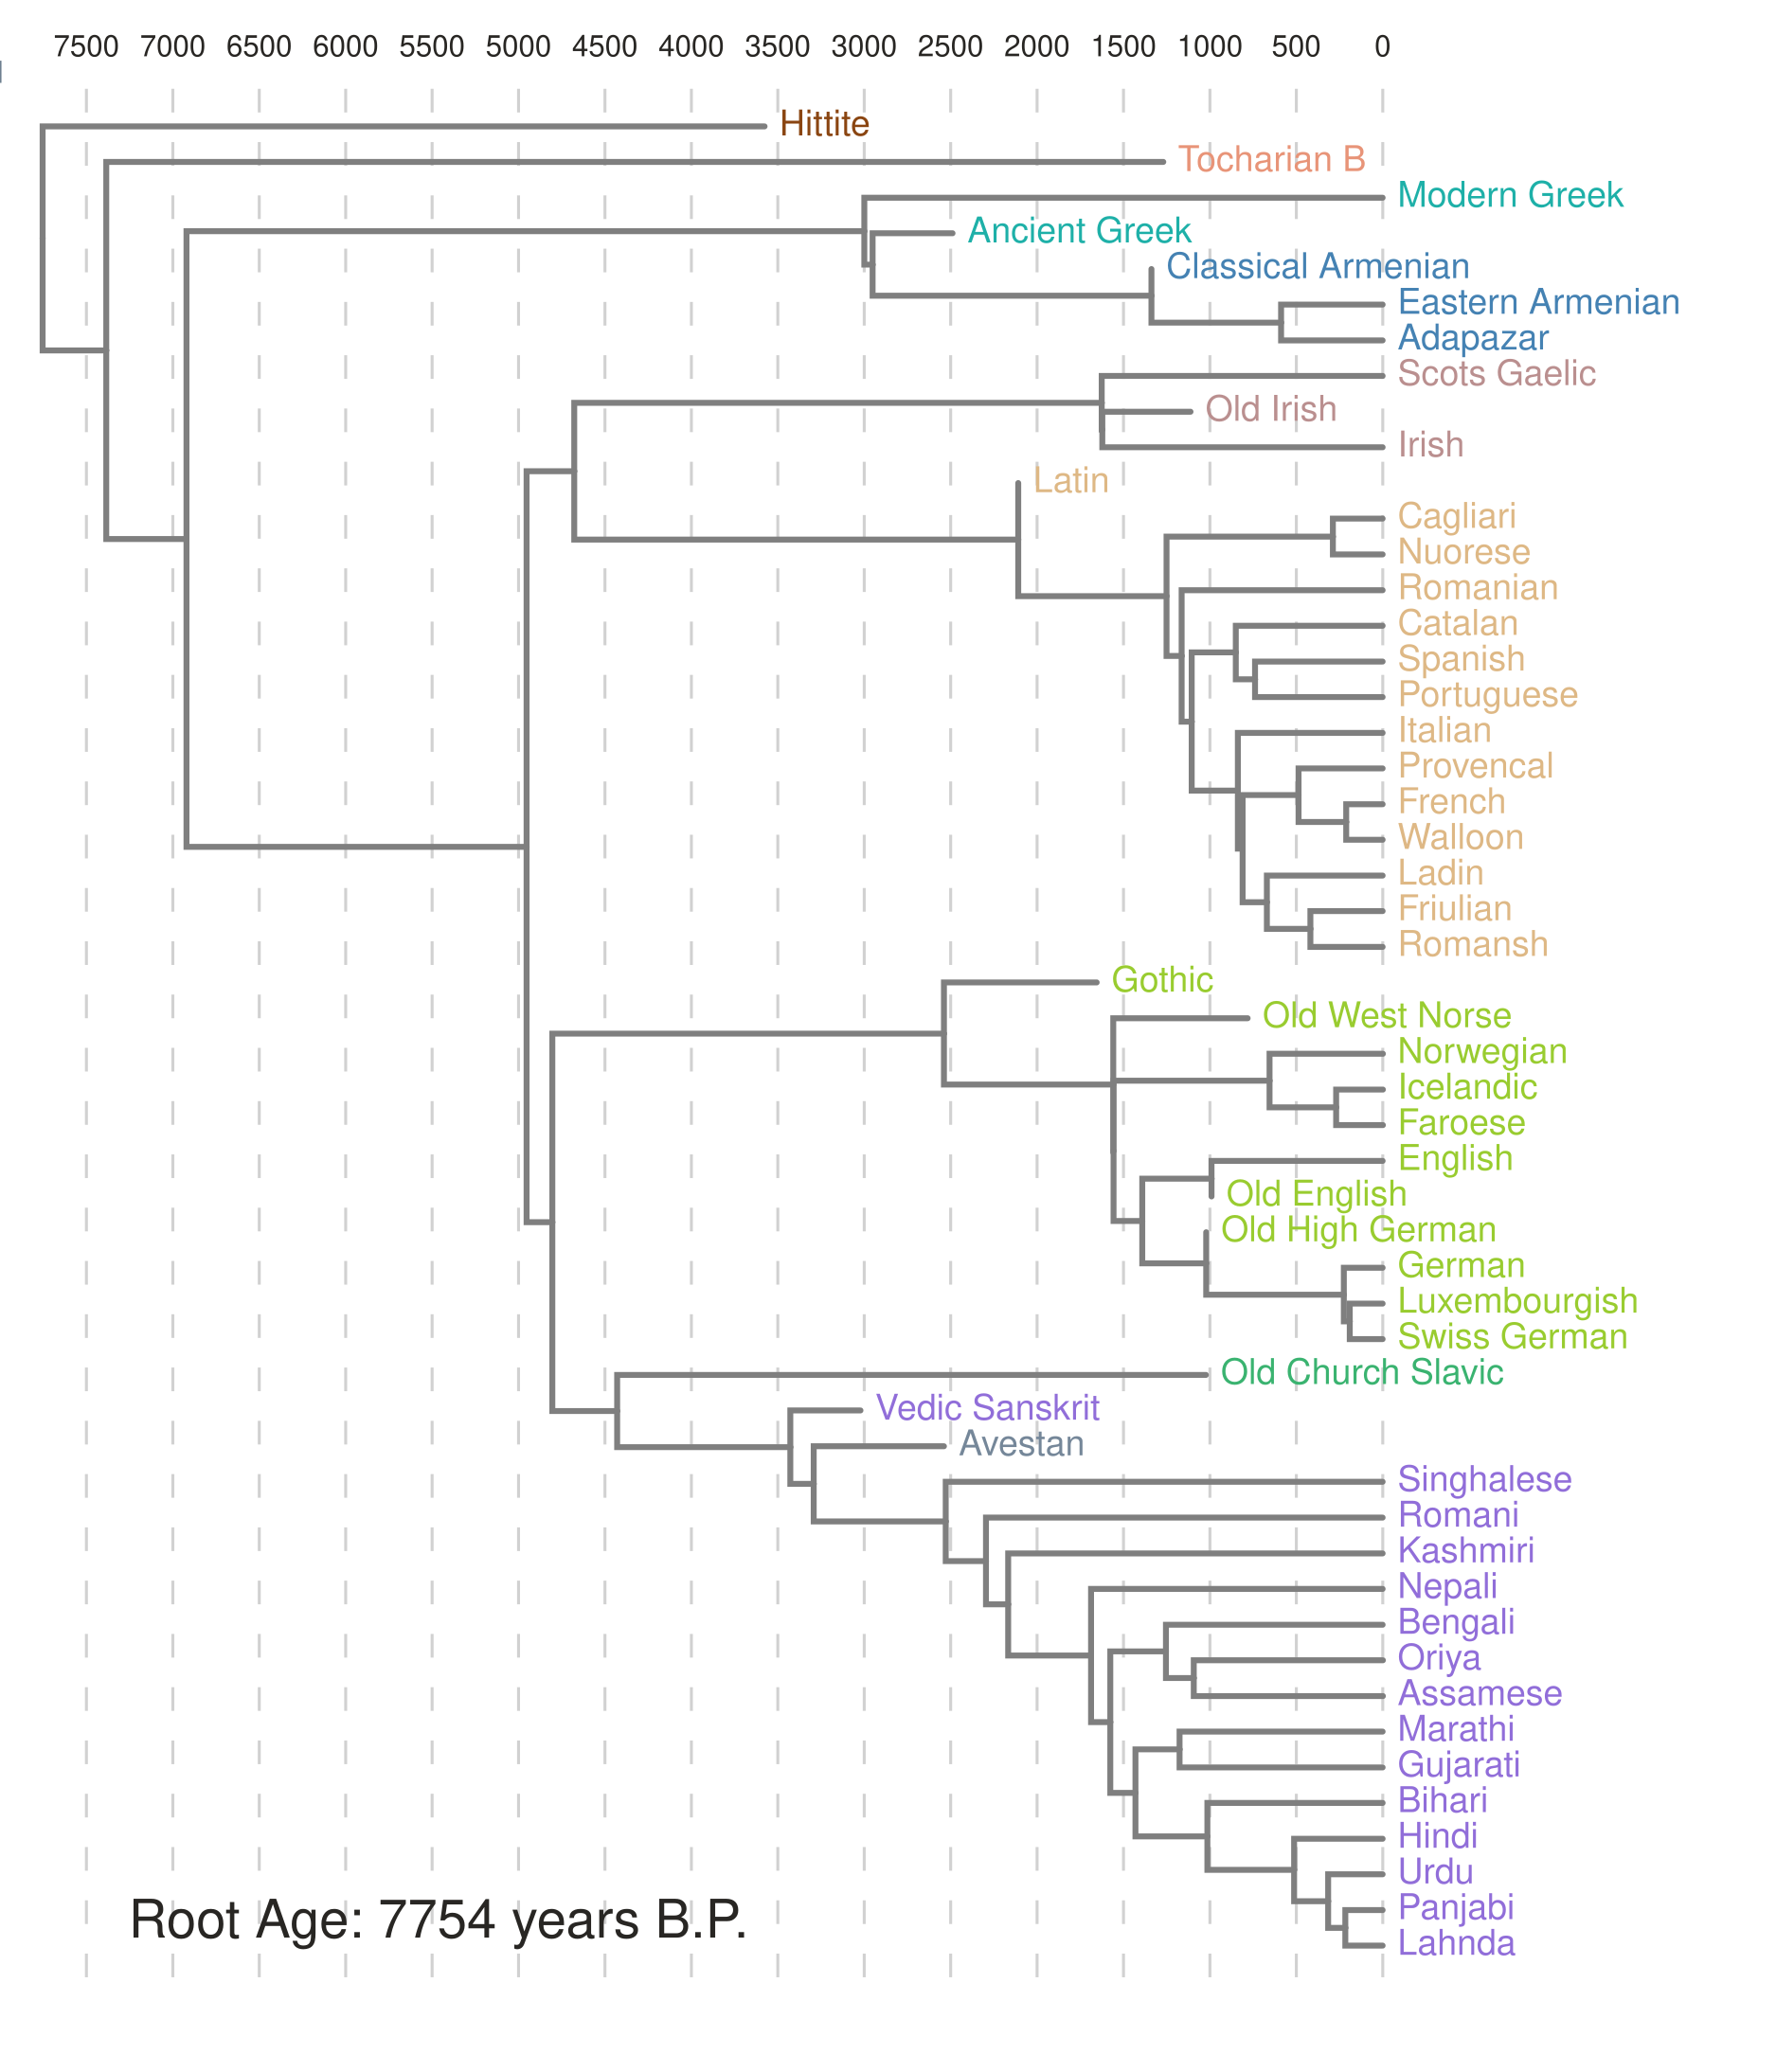
\includegraphics[width=\textwidth]{runs26-conv2}
         \label{fig:convtree2}
     \end{subfigure}
     \newline
     \begin{subfigure}[b]{0.4\paperwidth}
         \centering
         \caption{Phylogeny after 599,999 steps}
         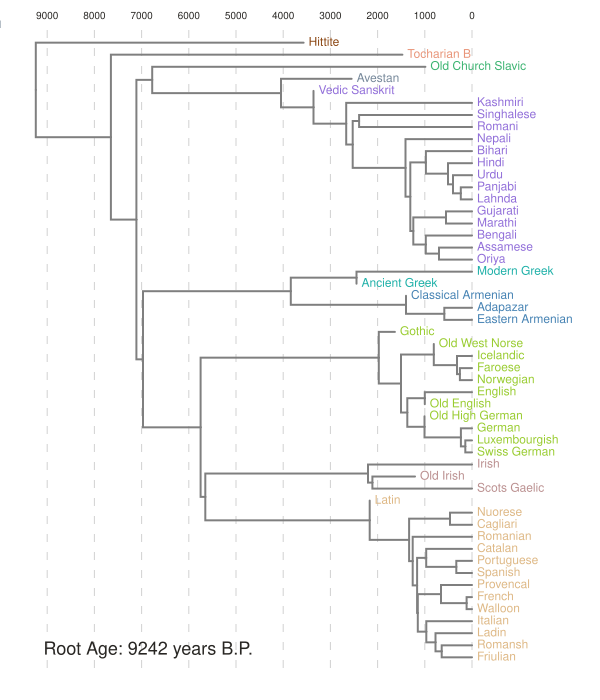
\includegraphics[width=\textwidth]{runs26-conv3}
         \label{fig:convtree3}
     \end{subfigure}
     \hfill
     \begin{subfigure}[b]{0.4\paperwidth}
         \centering
         \caption{Phylogeny after 999,999 steps}
         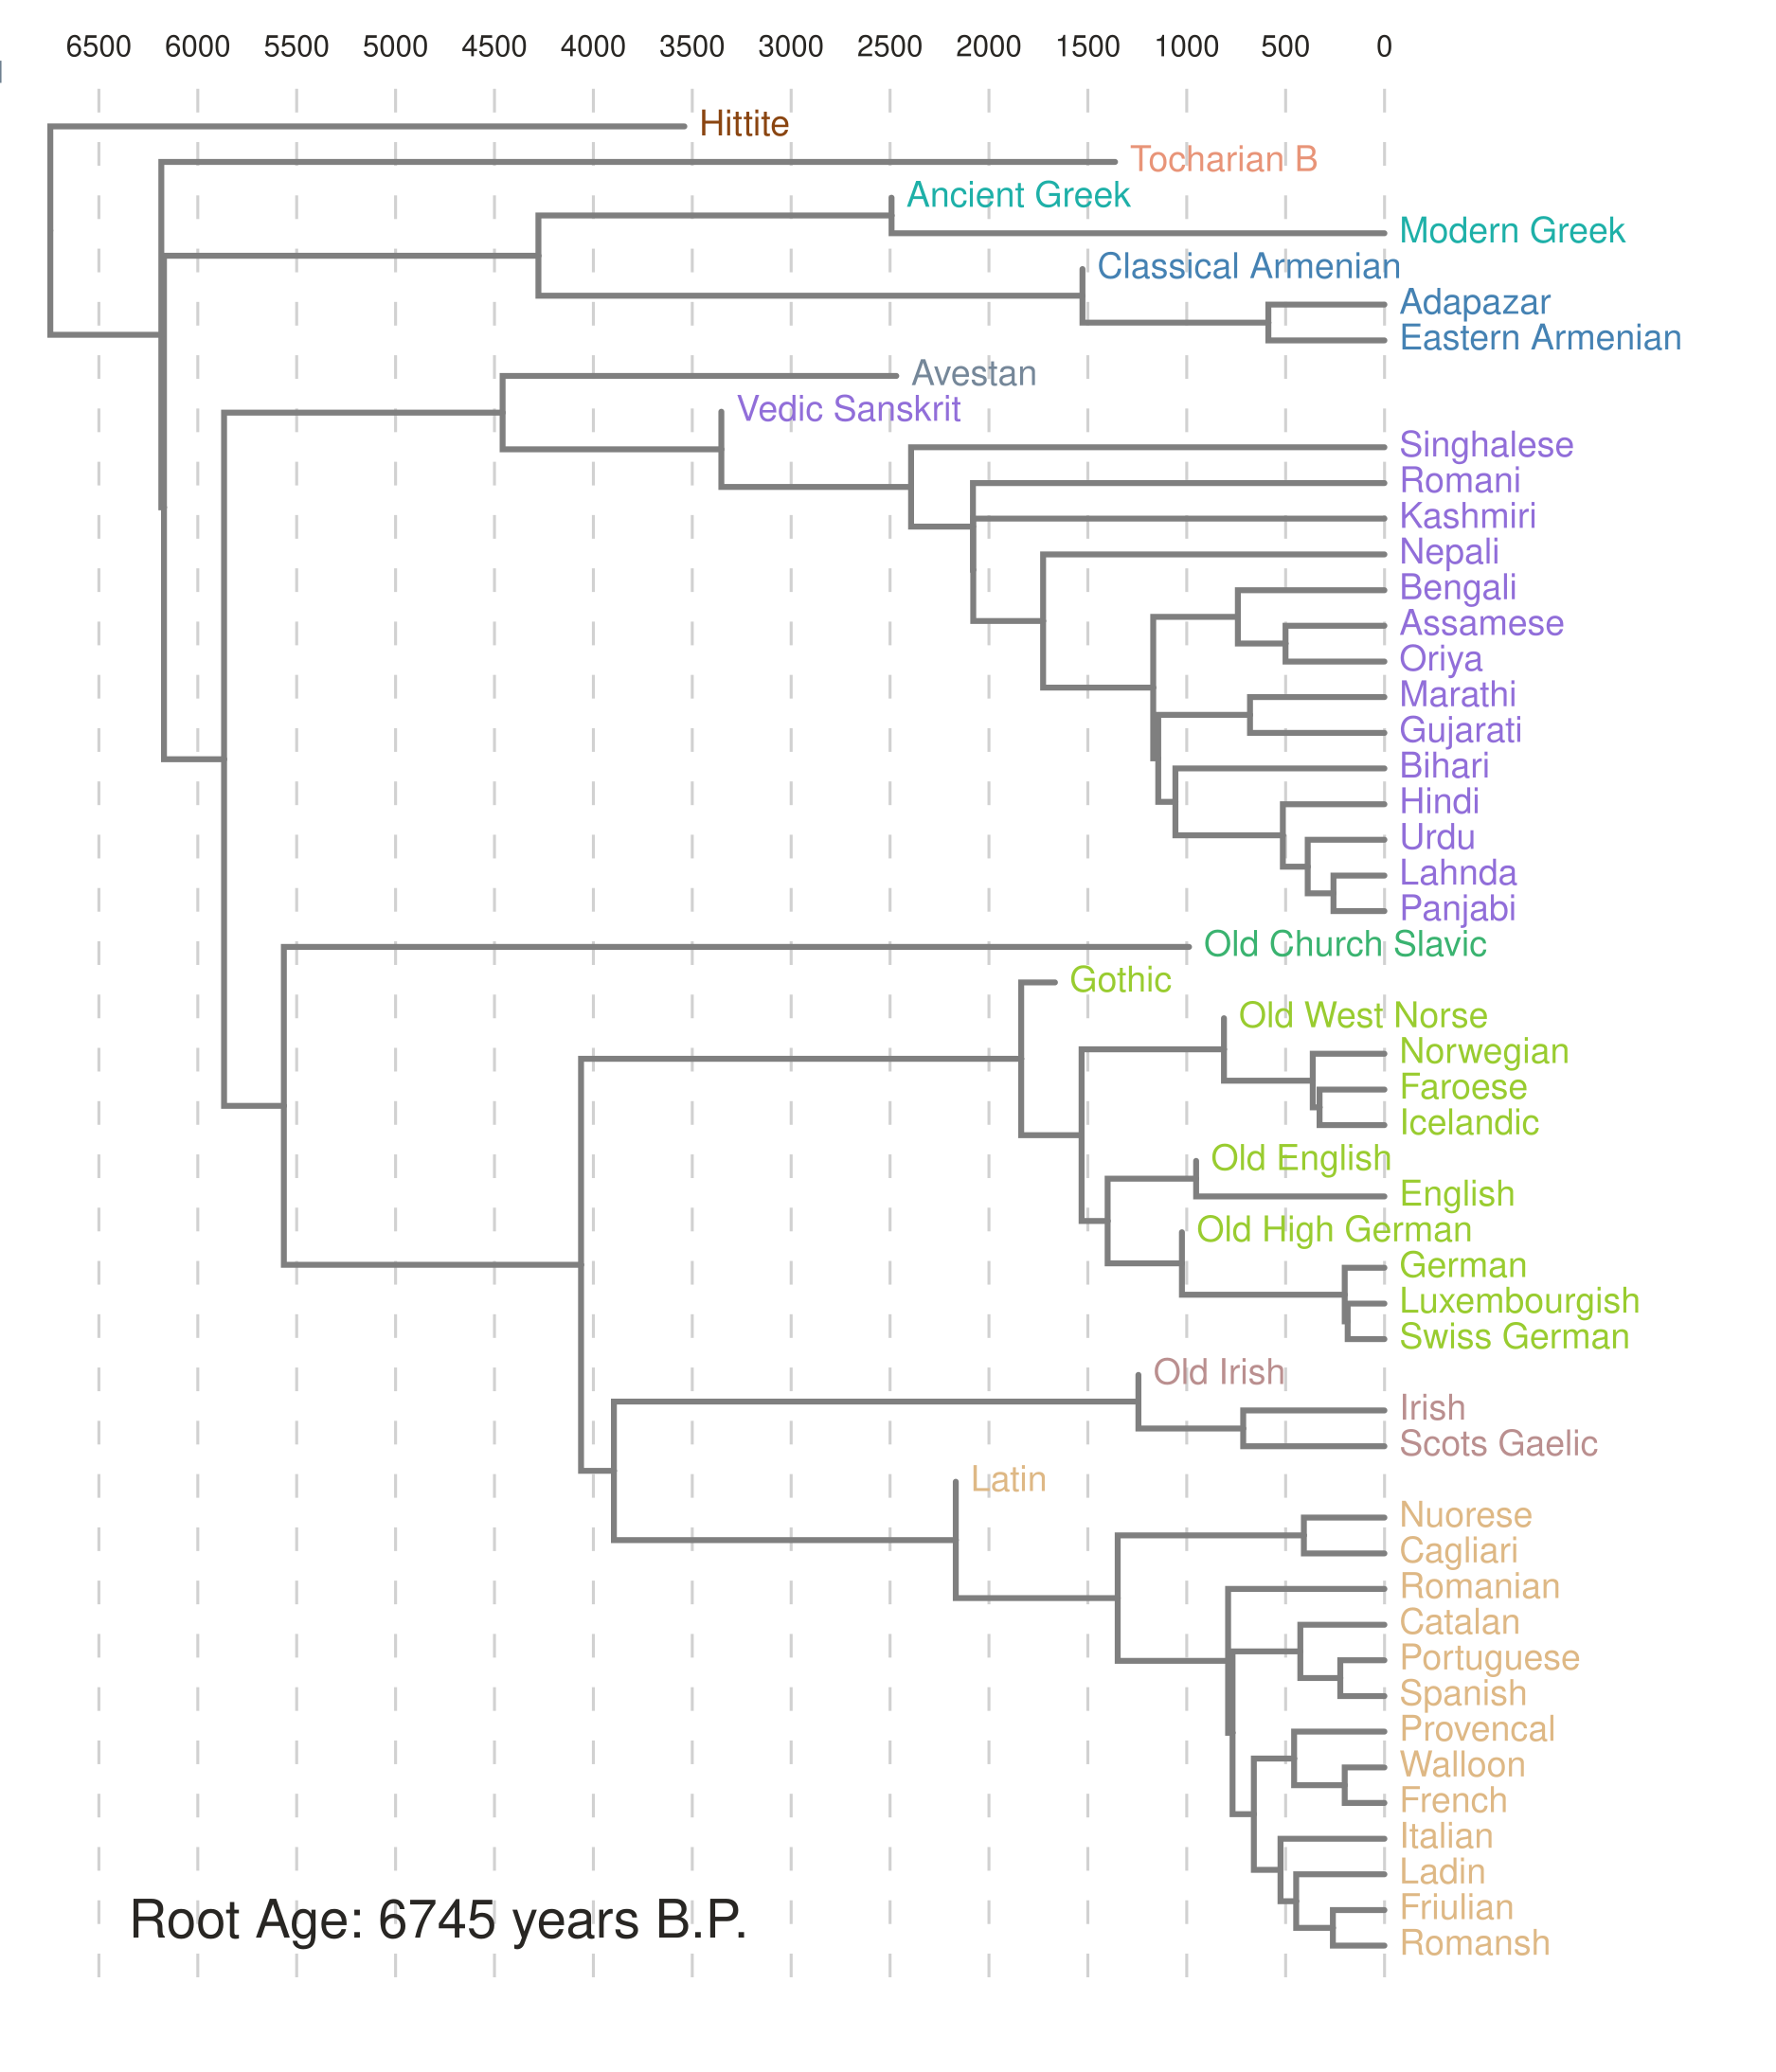
\includegraphics[width=\textwidth]{runs26-conv4}
         \label{fig:convtree4}
     \end{subfigure}
     \caption{Convergence towards the stationary distribution with the \textsc{Narrow} dataset}
     \label{fig:convtrees}
\end{figure*}

\subsection{Performance Analysis}

To investigate how implementation decisions impacted the performance of our software, we designed a benchmark test case. Our test case employs the \textsc{Narrow} dataset and the constant-population coalescent tree prior, with a chain length of 6 million steps, with tree snapshots taken after a burn-in period of 3 million steps.

In particular, we sought to determine the effectiveness of two specific optimisations. The first optimisation was our implementation of Damage-tracking, a system by which MCMC moves are able to inform the marginal likelihood logic which parts of the paramaterisation are affected by their choice of augmentation. The second optimisation was the usage of the BEAGLE library's CUDA backend, which allows marginal likelihood calculations to be performed in a highly parallel manner on an GPU.

We tested four software comfigurations, changing two variables: the BEAGLE platform, which was either the CPU backend or the GPU-accelerated CUDA backend; and the presence or absence of Damage-tracking. The test with CUDA and Damage-tracking corresponds to the configuration used in our main analyses.\footnote{CPU analyses were performed on the author's desktop computer, with an Intel i5-3570K processor running at 3.8 GHz. GPU analyses were performed on the Durham University NVIDIA CUDA Centre (NCC) cluster. NCC has been purchased through Durham University's strategic investment funds, and is installed and maintained by the Department of Computer Science.}

\begin{center}

\begin{tabular}{ |c|c|c| }
    \hline
    Platform & Damage & Runtime (mins) \\
    \hline
    CPU& Damage & 264 \\
    CPU& No Damage & 516 \\
    CUDA& Damage & 44 \\
    CUDA& No Damage & 82 \\
    \hline
\end{tabular}

\end{center}

The improvement gained by employing Damage-tracking is nearly a halving in runtime, a speedup which would likely be even higher on larger datasets. Meanwhile, the advantage of the CUDA backend over the CPU is even greater, providing a six-times speedup.

From these data it is evident that both Damage-tracking and the usage of the BEAGLE CUDA backend are significant performance optimisations that justify the extra effort in implementing the former, and in integrating the latter. In fact, these optimisations are so signficant that were it not for their combined speedups it would have made it difficult to perform the large analyses in this paper given the computational resources available to us.

\section{Evaluation}

Our work on \textit{Dyr} produced a final software solution implemented in approximately $3000$ lines of Rust program code.\footnote{Counted using the popular *nix utility \texttt{cloc}, excluding whitespace and comments.} The code is well-commented and free of technical debt, and is written in an appropriate and idiomatic fashion for the language and the problem domain.

We did not aim to compete with existing solutions for feature-completeness, and it is admittedly true that our software lacks some notable features such as ascertainment bias correction and a fossilised birth-death tree prior. However, as we have demonstrated, it is fully-featured enough to perform real-world phylolinguistic analyses, from which meaningful conclusions may be drawn, and produces results that are closely comparable to existing solutions.

One objective was for \textit{Dyr} to be high-performance, and as we have described, we have implemented powerful optimisations to achieve this goal. However, there is undoubtably more to do on this front. More fully-featured systems achieve better convergence and mixing by implementing considerably more MCMC moves, as well as dynamic tuning and support for multiple chains (so called `MCMCMC'). These features were out-of-scope for our research but would make positive additions to \textit{Dyr}, if they could be added without compromising the system's simplicity, elegance, and flexibility.

\subsubsection{Extensibility}
Moreover, we believe we have achieved a key goal, in producing a software package that is easily extensible. For example, let us consider the experience of a researcher aiming to implement a novel tree prior within \textit{Dyr}, as a case-study in extensibility and a demonstration of the clean abstractions engineered into the system.

Firstly, the programmer should add a case for the novel prior in the sum type\footnote{In Rust, sum types are called `enums', but this name is a little confusing -- users of other languages may know them as `tagged unions'.} \texttt{cfg::TreePrior}. The type \texttt{cfg::TreePrior::Novel} will act as a container for the pre-set configuration associated with the prior; for example, prior distributions for its parameters.

Next, the programmer should add a corresponding case for the novel prior in the sum type \texttt{params::TreePriorParams}. The type \texttt{params::TreePriorParams::Novel} will therefore hold a specific parameterisation of the tree prior. The design of \textit{Dyr} is such that the config wholly and neatly maps onto the parameter space in this manner.

Next, the programmer must add implementations for some specific functions relating to the tree prior. They need add a case to \texttt{TreePrior::draw()}, which selects an initial parameterisation at random from the pre-configured prior distributions. And naturally, they need also add a case to \texttt{TreePrior::log\_prior\_likelihood()}, which determines the log prior likelihood of a particular parameterisation under a particular tree prior model.

The programmer must create additional MCMC moves to suggest adjustments to the parameters of the novel prior. Creating a new move is as simple as defining a new heap-allocated type that implements the trait \texttt{Move} - i.e. has a function \texttt{make\_move} that accepts the current \texttt{Parameters} and mutates it, returning a \texttt{MoveResult}. Then, all that remains to do within \texttt{fitzroy} is to add a small piece of logic in \texttt{Configuration::get\_moves()} so that the proposal distribution includes these moves in the case of a run being configured with the novel prior.

Finally, the programmer should make some modest changes to the manifest parser so that the novel prior can be specified within the manifest format.

Provided that the novel tree prior is compatible with the binary-tree model of lingistic divergence, then making these augmentations is sufficient to implement it as a first-class citizen within \textit{Dyr}. We hope it is evident from this exposition that there is little-to-no confusing or tiresome boilerplate required; by-and-large the work required is simply that of implementing the core logic, with the powerful type system and intelligent abstractions handling the rest of the plumbing.

\section{Conclusion}\label{sec:conclusion}

In this paper we have taken a whistle-stop tour through the history of comparative linguistics, described the classic problem of the Indo-European \textit{Urheimat}, and outlined the history of MCMC algorithms in general and their application to phylogenetics and phylolinguistics in particular. We have described in detail the principles of every aspect of phylolinguistic inference, discussed the relative importance and merit of different model choices, in particular their reconcilability with linguistic realities.

Having laid a solid theoretical foundation, we have discussed the principles, structure, and implementation of \textit{Dyr}, our greenfield phylolinguistic inference solution. We have paid particular attention to the optimisations necessary to perform large real-world inferences without making unreasonable resource demands.

We have stress-tested our system by using it to tackle the established Indo-European problem-domain. We have demonstrated that our system produces similar results to established software, when performing similar analyses, while through our novel analyses we have contributed new evidence to the established body of research in this field.

We have demonstrated that our software has desirable convergence and performance characteristics that make it suitable for usage in serious practical applications, and finally, we have suggested how it may be easily and cleanly extended, thus serving as a platform for future research and investigation.

\subsubsection{Personal Reflections}

The tangible products of any endeavour are, except in cases of great artistry or genius, crude reflections of rather more sublime constructs in the mind of the practicioner. So it goes with this project. Pleased as I am with the software I have written, I am more satisfied still with the deep understanding I have gained for how complex phylogenetic inference systems operate.

Although they are, in point of fact, wholly mathematical entities, such systems are in character very mechanical; one can almost conceive of them as being formed of gears and springs, all finely meshed and interdependent -- more akin to a watch mechanism than an integrated function. And though one might \textit{know} how a mechanical watch works, it is established that to \textit{understand} such a device one must actually piece it together and feel it come to life in ones hands.

To phylogenetic inference, I believe the same applies; I do not believe that I could have attained my present understanding without having sought to write an inference system more-or-less from the ground up. The experience has been challenging and edifying in equal parts, and though I cannot claim great artistry or genius, I hope that the \textit{Dyr} program manifests at least a little of this profound learning.

\bibliographystyle{ieeetran}
\bibliography{dyr}

\end{document}
